\chapter{Applications}\label{chap2}

Mumford\pageoriginale et al. \cite[Chap.~2]{keyTE}
generalized the notion of 
tours embedding to that of \textit{toroidal embeddings}. Using this
they proved, among other things, the important semi-stable reduction
theorem is characteristic 0. Here we are concerned with more elementary
applications of tours embedding.  


In this chapter we restrict ourselves to tours embedding over the
field $\mathbb{C}$ of complex numbers, although some of the
result have interesting analogues over fields with non-archimedean rank
one valuation. 

\setcounter{section}{9}
\section{Manifolds with corners associated to torus
  embeddings}\label{chap2:sec10} 

Let $U(1)=\{z \epsilon  \mathbb{C}$; $\mid z \mid =1 \}$ be the
$I$-dimensional unitary group, i.e. $I$-dimensional real torus. Then the
$r$-dimensional algebraic torus $T=(\mathbb{C}^*)^r$ has the
$r$-dimensional real torus $CT = (U(1))^r$ as the maximal compact
subgroup such that  
$$
T/CT\cong (\mathbb{R}_{>0})^r \cong \mathbb{R}^r
$$
where $\mathbb{R}_{>_0}$ is the multiplicative group of positive real
numbers. 

Here is a coordinates-free description, which will be useful for torus
embeddings. Recall that $\mathbb{R}_0$ is the set of non-negative real
numbers. We have the valuation 
$$
 \ord : \mathbb{C} \xrightarrow{\quad | \quad | \quad } \mathbb{R}_0
 \xrightarrow[\sim]{-\log} \mathbb{R}\cup\{\infty\} 
$$
which\pageoriginale induces a homomorphism 
$$
 \ord : \mathbb{C}^* \xrightarrow{ \quad | \quad | \quad } \mathbb{R}_{>_0}
 \xrightarrow[\sim]{-\log} \mathbb{R}. 
$$

\noindent
Let $N \cong \mathbb{Z}^r$ be a free $\mathbb{Z}$-module of rank $r$
and let $M$ be its dual. Then as in \S. \ref{chap1:sec1} 
$$
T_N= N \otimes_\mathbb{Z}\mathbb{C}^* =\Hom_{gr}(M,\mathbb{C}^*) 
$$
is an $r$-dimensional algebraic torus over $\mathbb{C}$.

\begin{defi*}
We denote by $CT_N$ the compact (real) torus 
$$
CT_N=N\otimes_\mathbb{Z}U(1)=\Hom_{gr}(M,U(1)).
$$
\end{defi*}

The valuation ord applied to the second factor thus induces a
surjection 
\begin{align*}
\ord:T_N = \Hom_{gr}(M,\mathbb{C}*)&\xrightarrow{ \quad | \quad | \quad
}\Hom_{gr}(M, \mathbb{R}_{>_0})\\
&\xrightarrow[\sim]{-\log}
\Hom_{gr}(M, \mathbb{R})=N_{\mathbb{R}} 
\end{align*}
whose kernel is $CT_N$, thus we have 
$$
 \ord:T_N/CT_N\xrightarrow[\sim]{~}  N_{\mathbb{R}}. 
$$

Let $(N,\triangle)$ be an r.p.p.decomposition. Then $CT_N$ acts on the
corresponding tours embedding $T_N \emb(\triangle)$ endowed with the
\textit{classical\break (Hausdorff) topology} instead of the Zariski
topology. We then adopt the following definition for the notion
introduced by Mumford et al. \cite[Chap. 1,
  \S. 1]{keySC}.  

\begin{defi*}
We denote by
$$
\ord:T_N \emb(\triangle)\to Mc(N,\triangle)=T_N \emb(\triangle)/CT_N 
$$
the quotient space with respect to the classical topology and call it
the \textit{manifold with corners} associated to $T_N \emb(\triangle)$ 
\end{defi*}

It is\pageoriginale indeed a manifold with corners in the usual sense
(cf. Borel-Serre \cite{keyBS}) if  $T_N \emb(\triangle)$ is non-singular. By
Theorem \ref{chap1:thm4.2}, $T_N \emb(\triangle)$ is the union of
affine open sets   
$$
U(\sigma)=\Hom_{unit.semigr}(\check{\sigma}\cap M,\mathbb{C})
$$
with $\sigma$ running through $\triangle$, hence $Mc(N,\triangle)$ is the
union of its open sets 
\begin{align*}
\ord: U(\sigma)/CT_N &\xrightarrow[\sim]{\quad | \quad | \quad
}\Hom_{u.s.g}(\check{\sigma}\cap 
M, \mathbb{R}_o)\\
&\xrightarrow[\sim]{-\log}\Hom_{u.s.g}(\check{\sigma}\cap
M, \mathbb{R} \cup \{\infty\}). 
\end{align*}
The second description shows that $U(\sigma)/CT_N$ is isomorphic to
$( \mathbb{R}_o)^s \times(\mathbb{R}_{>_o})^{r-s}$ for some $s$ if
$\sigma$ is non-singular.  

\begin{prop}\label{chap2:prop10.1}
For an r.p.p.decomposition $(N,\triangle)$ the associated\break manifold with
corners $Mc(N,\triangle)$ has an action of $N_{\mathbb{R}}=
\mathbb{R}\otimes_{\mathbb{Z}}N$ 
and  is an equivariant partial compactification of $N_{\mathbb{R}}$
with the orbit decomposition. 
$$
Mc(N,\triangle)=\coprod_{\sigma \epsilon \triangle} \orb (\sigma)/CT_N 
$$
such that
$$
\orb
(\sigma)/CT_N\xrightarrow[\sim]{\ord}N_{\mathbb{R}}/(\mathbb{R}-\text{subspace
  generated by  }\sigma). 
$$
In particular
$$
\dim_{\mathbb{C}} \orb(\sigma)=\dim_{\mathbb{R}} \orb (\sigma)/CT_N=
    {\rm rank} N-\dim\sigma .
$$
\end{prop}

\begin{proof}
The  first part is obvious, since $Mc(N,\triangle)$ has an action of\break
$T_N/CT_N=N_{\mathbb{R}}$. Since $\orb(\sigma)=\Hom_{gr}(\sigma^\perp \cap
M,\mathbb{C}^*)$ by Theorem \ref{chap1:thm4.2}, we see that 
$$
\orb(\sigma)/CT_N\xrightarrow[\sim]{\orb}\Hom_{gr}(\sigma^\perp\cap
M,R)=N_R/(R-\text{ subspace $gen^d$ by }\sigma). 
$$

A map h:$(N,\triangle)\to (N',\triangle')$ of $r.p.p$. decompositions
obviously\pageoriginale gives rise to an equivariant continuous map
$$
Mc(h) : Mc (N, \triangle ) \to Mc (N', \triangle')
$$
\end{proof}

\begin{example*}[(Mumford)]
 Consider the projective line $\mathbb{P}_1 (\mathbb{C})$, which is the
 2-sphere in the classical topology. It corresponds to the
 r.p.p. decomposition $(N, \triangle) =
 (\mathbb{Z} \cdot \{\mathbb{R}_\circ, \{0\}, -\mathbb{R}_\circ\})$. 

$CT_N = U(1)$, and the orbits under it are the circles of the same
latitude. The quotient $Mc(N, \triangle)$ is the closed interval, a
compactification of the open interval isomorphic to
$N_{\mathbb{R}}=\mathbb{R}$. 
\begin{figure}[H]
\centering 
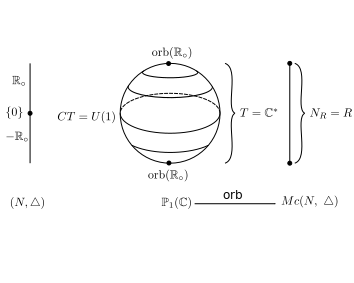
\includegraphics{vol58-fig/fig58-58.eps} 
\end{figure}
$$
(N, \triangle) \qquad \mathbb{P}_1 (\mathbb{C}) \xrightarrow{\ord} Mc
(N, \triangle)  
$$
\end{example*}

\begin{example*}
For a 2-dimensional $(N, \triangle), Mc(N, \triangle)$ looks like this  
\begin{figure}[H]
\centering 
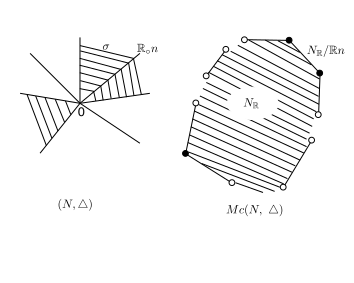
\includegraphics{vol58-fig/fig58-59.eps} 
\end{figure}
 
We\pageoriginale encounter many other examples later in \S
\S. \ref{chap2:sec11}, \ref{chap2:sec13}, \ref{chap2:sec14}, 
\ref{chap2:sec15}. Since the decomposition of $Mc (N, \triangle)$ into
$N_{\mathbb{R}}$-orbits faithfully reflects the incidence among the
$T_N$-orbits of $T_N$ emb $(\triangle)$ the pictures we can draw of
$Mc (N, \triangle)$ in dimensions 2 and 3 will  give us a good
geometric insight. 
\end{example*}

\begin{remark*}
Over a field $k$ with a non-archimedean rank one valuation
$$
\ord : k \to \mathbb{R} \cup \{ \infty \}, 
$$
we have an obvious analogue of $Mc (N, \triangle)$.
\end{remark*}

Although the following description of the fundamental group has
nothing to do with the manifolds with corners, we state it here, since
it will be very convenient later. 

\begin{prop}[Mumford]\label{chap2:prop10.2}
Let $(N, \triangle)$ be an r.p.p.decomposition and let $T_N \emb
(\triangle)$ be the corresponding torus embedding over 
$\mathbb{C}$ endowed with the classical topology. Then we have the
following canonical description of the fundamental group. 
$$
\pi_1 (T_N \text{emb} (\triangle)) = N/ (\text{the subgroup
  gen}^{\underline{d}} \bigcup_{\sigma \in \triangle} (\sigma \cap
N)). 
$$
\end{prop}

\begin{proof}
For  simplicity, let $T=T_N$ and $X = T_N \emb (\triangle)$. We have a
well-known isomorphism 
$$
N \xrightarrow{\sim} \Hom_{gr} (U(1), T) = \pi_1 (T)  
$$
which sends $n \in N$ to the loop $U (1) \ni u \to u^{<?, ~ n>} \in
\text {Hom}_{gr} (M, \mathbb{C}^*)=T$, where\pageoriginale $\langle ,
\rangle : M 
\times N \to 
\mathbb{Z}$ is the dual pairing as before. By Theorem \ref{chap1:thm4.2}, $X$ is
covered by $U(\sigma) = \Hom_{u.s.g}(\check{\sigma} \cap M,
\mathbb{C}) \supset T$ with $\sigma$ running through $\triangle$. By
generalized van Kampen's theorem in Olum \cite{keyO1}, it is thus enough to
show that the canonical homomorphism 
$$
N = \pi_1 (T) \to \pi_1 (U(\sigma)) 
$$
is surjective with the subgroup $N$' generated by $\sigma \cap N$ as
the kernel. Note that $N'$ is a direct summand of $N$. 
\end{proof}

Since $U(\sigma)$ is non-canonically isomorphic to the product of the
algebraic torus $(N/N') \otimes_{\mathbb{Z}} \mathbb{C}^*$ and the
lower dimensional $T_{N'}$-embedding corresponding to $\sigma$
considered as a cone in $N'_R$, it is obviously enough to show that
$U(\sigma)$ is simply connected if $\sigma$ generates
$N_{\mathbb{R}}$. First of all, $N = \pi_1 (T)$ is mapped surjectively
onto $\pi_1 (U(\sigma))$, since $U(\sigma)-T$ is of real codimension
$\geq 2$ in $U(\sigma)$, by the so-called general position
argument. On the other hand, for $n \in \sigma \cap N$ and $0 \le
\varepsilon \le 1$, the map 
$$
U(1) \ni  u \mapsto (\varepsilon u)^{<?, n>} \in
\Hom_{u.s.g}(\check{\sigma} \cap M, \mathbb{C}) = U{\sigma}  
$$
establishes a homotopy which kills $n$ in $\pi_1 (U(\sigma))$ as
$\varepsilon$ goes to 0, since $<m, n> \geq 0$ for $m \in
\check{\sigma}\cap M$. Since $\sigma \cap N$ generates $N$ as a group,
we are done.  

For illustrative examples, we refer the reader to \S
\S. \ref{chap2:sec13}, \ref{chap2:sec14}.  


\section{Complex tori}\label{chap2:sec11} 
The following\pageoriginale ``multiplicative'' formulation of complex
tori and polarizations was given by Tate in his lecture in July
1967. It was used effectively by Mumford et al. \cite{keySC}. In this way,
we can also formulate their analogues in the non-archimedean case, or
even in the ideal-adic case. (cf. Morikawa \cite{keyM5}, McCabe \cite{keyM2},
Mumford \cite{keyM7} and Gerritzen \cite{keyG1}.)  

Given a $g$-dimensional complex torus $X$, there exists a symmetric $g
\times  g$ matrix $\tau = (\tau_{jk})$ with the positive definite imaginary
part $\im(\tau)$ such that 
$$
X = \mathbb{C}^g / (\mathbb{Z}^g + \mathbb{Z} \tau_1 + \cdots +
\mathbb{Z}\tau_g) 
$$
where $\tau_1, \ldots , \tau_g$ are the row vectors of $\tau$. We have
a surjective homomorphism 
$$
\mathbb{C}^g \to (\mathbb{C}^*)^g
$$
sending $(z_1, \ldots , z_g)$ to $(\exp (2\pi i z_1), \ldots , \exp (2
\pi i z_g))$.  

\noindent
Let $\Gamma$ be the image of the lattice, which is a free abelian
subgroup of $(\mathbb{C}^*)^g$ of rank $g$ such that  
$$
X = (\mathbb{C}^*)^g/\Gamma.
$$
This description is very efficient, since it gets rid of the
redundancy $\mathbb{Z}^g$. It also fits in nicely with torus
embeddings and will give us good insight into the construction of
degenerating families. Here is the \textit{coordinate-free} approach: 

Let\pageoriginale $N \cong \mathbb{Z}^g$ be a free abelian group of
rank $g$ with the dual $M$. As before, let $T = T_N = \Hom_{gr}(M,
\mathbb{C}^*)$ be the algebraic torus.   

\begin{defi*}
A {\em period } for $T = \Hom_{gr} (M, \mathbb{C}^*)$ is a
homomorphism  
$$
q : \Gamma \to T, \quad \gamma \mapsto q^\gamma 
$$
from a free $\mathbb{Z}$-module $\Gamma$ of rank $g$, which is
injective with compact cokernel $X =  T/q^\Gamma$, a complex torus. 
\end{defi*}

Composed with the valuation $\ord (?) = - \log |?| :
\mathbb{C}^* \to \mathbb{R}$, $q$ gives rise to a homomorphism 
$$
\ord \circ q : \Gamma \to N_{\mathbb{R}} = Mc (N, \{ 0 \}). 
$$

The injectivity and the compactness of the cokernel of $q$ are
equivalent to those of $\ord \circ q$. 

For $\gamma \in \Gamma$ and $m \in M$, let $Q (\gamma, m) =
q^{\gamma} (m) \in \mathbb{C}^*$. Thus we have a non-degenerate
biadditive pairing 
$$
Q : \Gamma \times M \to \mathbb{C}^*.
$$

\begin{defi*}
For a period $q : \Gamma \to T = \Hom_{gr} (M, \mathbb{C}^*)$,
let 
$$
\hat{q} : M \to \hat{T} = \Hom_{gr} (\Gamma, \mathbb{C}^*) 
$$
be the period given by $\hat{q}^m (\gamma) = q^\gamma (m)$. We call
$\hat{X} = \hat{T}/\hat{q}^M$ the {\em dual complex torus}. 
\end{defi*}

Recall that $m \in M$ gives rise to the character $T \ni t \mapsto
e(m) (t) \in \mathbb{C}^*$ (cf. \S. \ref{chap1:sec1}). Consider the
\textit{formal 
  Laurent series} 
$$
\theta (t) = \sum_{m \in M} a_m e(m) (t) 
$$
for $t \in T$ and $a_m \in \mathbb{C}$. The following is well-known: 

\begin{prop}\label{chap2:prop11.1}
The ring\pageoriginale $Ho1(T)$ of holomorphic functions consists of the Laurent
series which are convergent everywhere on $T$. The units in $Ho1(T)$
are of the form 
$$
ae(m) \quad \text{for} \quad  a \in \mathbb{C}^* \quad  \text{and}
\quad   m \in M. 
$$
\end{prop}

It is also well-known that the \textit{positive divisors} on the
complex torus $X = T/q^\Gamma$ are in one to one correspondence with
the $\Gamma$-invariant positive divisors on $T$, which are of the form
div$ (\theta)$ for $ 0 \neq \theta \in Ho1 (T)$. From what
we saw above, the $\Gamma$-invariance means that there exist maps 
$$
c : \Gamma \to \mathbb{C}^* \quad \text{and}\quad \Gamma \to M 
$$
such that
\begin{equation*}
\theta (q^\gamma t) c (\gamma) t^{\alpha(\gamma)} = \theta (t) \text {
  for all } \gamma \in \Gamma. \tag{*} 
\end{equation*}
Such $\theta (t)$ is called a \textit{theta function}. We see
immediately the following: 

\setcounter{lemma}{1}
\begin{lemma}\label{chap2:lem11.2}%%% 11.2
The pair $(\alpha, c)$ satisfies the following conditions and is
called a \textit{theta type} for the period $q$. 
\begin{enumerate}[(i)]
\item $\alpha : \Gamma \to M$ is a $Q$-symmetric homomorphism, i.e.
$$
\alpha(\gamma + \gamma') = \alpha (\gamma) \cdot \alpha(\gamma') \quad
\text{and} \quad  Q(\gamma', \alpha(\gamma)) = Q(\gamma, \alpha(\gamma')).
$$

\item $c : \Gamma \to \mathbb{C}^*$ is a quadratic character with
  respect to $Q (?, \alpha(?))$, i.e. 
$$
c(\gamma + \gamma')/c(\gamma)c(\gamma') = Q(\gamma, \alpha
(\gamma')). 
$$
\end{enumerate}
\end{lemma}

Given theta functions $\theta (t)$ and $\theta' (t)$ with the theta
types $(\alpha, c)$ and $(\alpha', c')$, respectively, we see that
$\theta (t) \theta' (t)$\pageoriginale is of the theta type $(\alpha +
\alpha', cc')$. Moreover, $\divv(\theta)$ and div $(\theta')$ give rise
to linearly equivalent divisors on $X$ if and only if there exists $m \in
M$ such that  
$$
\alpha' = \alpha \quad \text{and} \quad c' = c \cdot Q (?, m). 
$$ 
Thus we conclude:

\setcounter{prop}{2}
\begin{prop}\label{chap2:prop11.3}
We have an isomorphism 
$$
\text{Pic}(X) = \{\text{theta types } (\alpha, c) \} /\{ (0, Q (?,
m)) ; m \in M \}  
$$
and an exact sequence 
$$
0 \to \hat{X} \to \text{ Pic }(X) \to \Hom_{Q-symm} (\Gamma,
M) \to 0. 
$$
\end{prop}

Given a theta type $(\alpha, c)$, let $\Gamma (\alpha, c)$ denote the
corresponding line bundle on $X$. 

\begin{prop}\label{chap2:prop11.4}
Given a theta type $(\alpha, c)$ for $q$, we have a homomorphism
$$
\Lambda (L (\alpha, c)) : X \to \hat{X} 
$$
induced by $\circ \alpha : T = \Hom_{gr}(M, \mathbb{C}^*) \to
\hat{T} =  \Hom_{gr} (\Gamma, \mathbb{C}^*)$.  
\end{prop}

\noindent
 (1) $\alpha : \Gamma \to M$ is injective if and only if ord $\circ
Q(?, \alpha (?)) : \Gamma \times \Gamma \to \mathbb{R}$ is
non-degenerate. In this case, $\Lambda(\alpha, c))$ is an isogeny
whose degree is equal to the order deg$(\alpha)$ of coker [$ \alpha :
  \Gamma \to M$], and $L (\alpha, c)$ is called \textit{
  non-degenerate}. 

\noindent
$(2)$ If, moreover, ord $\circ Q (?, \alpha (?)) : \Gamma \times \Gamma \to
\mathbb{R}$ is positive definite, then $L (\alpha', c)$ is an ample
line bundle, and $\alpha$ is called a \textit{polarization}. In this
case, the theta functions of the theta type $(\alpha, c)$ form a
$\mathbb{C}$-vector space of dimension $\deg (\alpha)$.\pageoriginale The
polarization is \textit{principal} if and only if  
$$
\alpha : \Gamma \overset{\sim}{\to}M, \quad \text{i.e.} \quad \Lambda
(L(\alpha, c)) : X \overset{\sim}{\to} \hat{X}.  
$$

When we have a principal polarization $\alpha$ on $X$, we can identify
$\Gamma$ with $M$ via $\alpha$. Thus a principally polarized
$g$-dimensional complex torus $X$ is determined by a symmetric
biadditive map 
$$
Q : M \times M \to \mathbb{C}^* 
$$
with $P = \ord \circ Q : M \times M \to \mathbb{R}$ positive
definite so that 
$$
X = T/ \{ Q (m, ? ) ; m \in M \}.  
$$


Let us fix $M = \mathbb{Z}^g$ with the $\mathbb{Z}$-basis $\{m_1,
\ldots , m_g \}$. Let  
\begin{equation*}
PdSym (M \times M, \mathbb{C}^*) =  \left\{
\begin{minipage}{6.5cm}{
 symmetric biadditive  $Q : M \times M \to \mathbb{C}^*$ 
with ord $\circ Q $ positive definite}
 \end{minipage}
 \right \}
\end{equation*}

We then have a \textit{versal family} over $PdSym (M \times  M,
\mathbb{C}^*)$ of principally polarized $g$-dimensional complex tori,
whose total space is the quotient of $T \times PdSym (M \times M, \mathbb{C}^*)$,
with $T= \Hom_{gr} (M, \mathbb{C}^*)$, by the action of $M$ defined by 
$$
(t, Q) \mapsto (Q (m, ?) t, Q) \quad \text{for} \quad  m \in M.
$$

$Pdsym (M \times M, \mathbb{C}^*)$ is an open subset of 

Sym $(M \times M, \mathbb{C}^*$ = \{symmetric biadditive $Q : M \times M \to
\mathbb{C}^*$\}, which, by component wise multiplication, is a
$g(g+1)/2$-dimensional algebraic torus over $\mathbb{C}$ with the
character group 

$S^2 (M) =$\pageoriginale the symmetric product of $M$ of degree 2 and
the group of one parameter subgroups  
$$
\text{Sym}(M \times  M, \mathbb{Z}) = \{ \text{symmetric bilinear maps} M \times
M \to \mathbb{Z}\}.  
$$

As usual, let $S_g$ be the Siegel upper half plane of complex
symmetric $g x g$ matrices $\tau = (\tau_{jk}) $ with the positive
definite imaginary part $Im(\tau) > 0$. Then an element  
$$
\begin{pmatrix}
A & B \\
 C & D 
\end{pmatrix}
$$
of the Siegel modular group $Sp_g(\mathbb{Z})$ acts on $S_g$ via $\tau
\mapsto (A\tau + B)(C\tau + D)^{-1}$. The map $\tau \mapsto Q$ defined
by  
$$
Q(m_j, m_k ) = \exp (2\pi i\tau_{jk}) 
$$
establishes an embedding
$$
S_g/\{ \begin{pmatrix} 1 & B \\ 0 & 1 \end{pmatrix} \in Sp_g
(\mathbb{Z}) \} \xrightarrow{\sim} PdSym (M \times M, \mathbb{C}^*) \subset
Sym (M \times M, \mathbb{C}^*). 
$$

The first step in compactifying the moduli space of principally
polarized complex tori in Mumford et al. \cite{keySC} is to choose a nice
$Sym (M \times M, \mathbb{C}^*)$-embedding corresponding to an \textit{
  admissible} r.p.p.decomposition $(Sym(M \times M, \mathbb{Z}, \triangle)$
which  is invariant under the canonical action of Aut$(M) \cong GL_g
(\mathbb{Z})$ with $\triangle/\text{Aut} (M)$ finite and fills up the
convex hull in $Sym (M \times M, \mathbb{R})$ of the set of positive
semi-definite integral forms. 

The Delony-Voronoi decomposition is such  a decomposition and was used
by Namikawa \cite{keyN5} for his Delony-Voroni compactification of the
moduli space, over which he could even construct a
family\pageoriginale of what he calls \textit{stable quasi-abelian
  varieties}. Here is a brief coordinate-free account of the part
relevant to us:  

Let $P : M \times M \to \mathbb{R}$ be a positive semi-definite  bilinear
form. $P$ defines a pseudo-norm $|| x ||_p = P(x, x)^{1/2}$ on
$M_{\mathbb{R}}$. For $x\in M_\mathbb{R}$ let 
$$
w(x, P) = \{ m \in M ; || x - m ||_P = \min_{m' \in M} || x - m' ||_P
\}. 
$$

\noindent
The convex hull $D(x, P)$ in $M_{\mathbb{R}} $ of $w (x, P)$ is an
(unbounded if $P$ is not definite) polyhedron in $M_{\mathbb{R}}$ and
is called a \textit{Delong cell}. The set $Del(M_{\mathbb{R}}, P)$ of
Delony cells is the \textit{Delony decomposition} and is invariant
under the translation action of $M$.  

On the other hand,
\begin{gather*}
V (x, P) = \{ y \in N_\mathbb{R} ; \langle m' , y \rangle + P(m', m' +
2m) \ge \\ 
\hspace{3cm}
\text{for all } \; m' \in M \text{ and  all}  m \in w (x, P) \} 
\end{gather*}
is a polyhedron in $N_\mathbb{R}$ and is called a \textit{Voronoi
  cell}. Let  $P^* : M_\mathbb{R} \to N_\mathbb{R}$ be the canonical
linear map defined by $x' \mapsto P(x', ?)$. Then $V (x, P)$ is the
image under $-2P^*$ of $\{ x' \in M_\mathbb{R} ; || x' - m ||_P =
\min\limits_{m' \in M} || x' - m' ||_p$ for all $m \in w (x, P) \}$.
The set Vor$(N_\mathbb{R}, P)$ of Voronoi cells is the \textit{
  Voronoi decomposition} of the image of $P^* : M_\mathbb{R } \to
N_\mathbb{R}$ and is invariant under the translation action of $2P^*
(M)$. This is the original definition by Voronoi and is different from
the usual one, for  instance in Oda-Seshadri \cite{keyOS}. 

\begin{defi*}
Positive\pageoriginale semi-definite bilinear forms $P$, $P' : M \times M
\to \mathbb{R}$ are \textit{equivalent} if   
$$
\text{Del}(M_\mathbb{R}, P) = \text{Del} (M_\mathbb{R}, P'). 
$$
\end{defi*}

An equivalence class $\sum$ of positive semi-definite forms is a
polyhedral cone, a \textit{Delony-Voronoi cone}, in $Sym (M \times M,
\mathbb{R})$. Let Del-Vor be the set of such equivalence classes. Then
we have an admissible r.p.p.decomposition 
$$
(\text{Sym}(M \times M, \mathbb{Z}, \text { Del-Vor}),
$$
the \textit{Delony-Voronoi decomposition}, which is
Aut$(M)$-invariant with Del-Vor/Aut$(M)$ finite and which fills up the
convex hull of the set of positive semi-definite integral forms.  

On the other hand, for a Delony-Voronoi cone $\sum$ and a Delony cell
$D$ of the Delony decomposition common to forms in $\sum$, 
\begin{align*}
\sigma (\sum, D) =  (y, P) \in N_\mathbb{R} \times \sum ; &\langle m', y
\rangle + P(m', m' + 2m ) \ge 0 \\ 
&\text{ for all } m' \in M \text{ and all } m \in M \cap D  \bigg\} 
 \end{align*}
  is a polyhedral cone in $N_\mathbb{R} \oplus Sym (M \times M,
  \mathbb{R})$. The set Mixed of these cones, \textit{mixed cones},
  gives rise to an r.p.p.decomposition 
 $$
 (N \oplus \text{Sym}(M \times M, \mathbb{Z}), \text{ Mixed}) 
 $$
 called the \textit{mixed decomposition}.
 
 The second projection induces a map of r.p.p.decompositions 
$$
p_2 :
  (N \oplus \text{ Sym }(M \times M, \mathbb{Z}), Mixed) \to (Sym (M \times M,
 \mathbb{Z}), Del-vor). 
$$\pageoriginale
 
 \noindent
 Thus we have an equivariant morphism of torus embeddings
 $$
\rho : T_{N \oplus\text{ Sym }(M \times M, \underset{\substack{||
       \\ \mathscr{X}}}{\mathbb{Z}}}  \emb (\text{Mixed}) \to T_{\text{Sym
   }(M \times M, \underset{\substack{|| \\ \mathcal{B}}}{\mathbb{Z}}}
 emb(Del-Vor)  
$$
a ``family of semi-universal coverings'' of Namikawa
\cite[\S.~8]{keyN5}.  
 
 For various reasons (cf. ibid. (13.8)), it is more convenient to
 consider the \textit{level} $2 \nu$ \textit{action} $(\nu \geq 1)$
 of the lattice $M$ on $\mathcal{B}$. It is induced by the action of
 $M$ on $N \oplus Sym (M \times M, \mathbb{Z})$ by  
 $$
 (y, P) \mapsto (y + P (2\nu m, ?), P) \quad \text{for} \quad  m \in M   
 $$
 which preserves the mixed decomposition. On $T \times $ PdSym $(M \times M,
 \mathbb{C}) \subset \mathcal{B}$, it coincides with the action 
 $$
 (t, Q ) \mapsto (Q (2\nu m, ?) t, Q) \quad \text{for} \quad m \in M.    
 $$
 
 Let $\mathscr{X}^\circ \subset \mathscr{X} $ be the interior of the
 closure of PdSym $(M \times M, \mathbb{C}^*)$. Then
 $\mathcal{B}^{\circ} = \rho^{-1} (\mathscr{X}^\circ)$ is the inverse
 image under ord of the 
 open set in $Mc (N \oplus \text{ Sym }(M \times M, \mathbb{Z})$, Mixed)
 consisting of $N_\mathbb{R} \times $ PdSym $(M \times M, \mathbb{R})$ and the
 boundary at infinity. 
 
 The level $2 \nu$ action of $M$ induced on the open set, hence also
 its action on $\mathcal{B}^\circ$, is properly discontinuous and
 fixed point free. Thus we have a family  
 $$
\omega^{(\nu)} : a^{(\nu)} = B^\circ /  (\text{level $2 \nu$ action of
 $M$}) \to \mathscr{X}^\circ
$$ 
  of ``stable quasi-abelian varieties of dimension $g$ and of degree
  $\nu$'' of Namikawa \cite[\S.~13]{keyN5}. 

 We now\pageoriginale look more specifically at \textit{one parameter
   degenerations} of principally polarized $g$-dimensional complex
 tori which was studied in detail by Mumford \cite{keyM7}, Nakamura 
 \cite{keyN3},  \cite{keyN4} and Namikawa \cite[\S.~17]{keyN5}. See
 also Namikawa \cite{keyN6} for 
 toroidal degenerations.  

\begin{defi*}
We denote by $U = \{ \lambda \in \mathbb{C} ; | \lambda | < 1\}$ the
open unit disk and $U^* = U - \{ 0 \}$ the punctured disk. 
\end{defi*}

It will be more convenient later to think of $U^*$ and $U$ as open
sets in $T_{\mathbb{Z} \ell } ~\emb (\{\mathbb{R}_0 \ell, \{ 0 \} \})=
\mathbb{C}$ for a free $\mathbb{Z}$-module $\mathbb{Z}\ell$ of rank
one with the base $\ell$ with 
\begin{align*}
U & = \ord^{-l} (\mathbb{R}_{>0} \ell \amalg \{ \infty \} )\\
U^* & = \ord^{-l} ( \mathbb{R}_{>0} \ell )
\end{align*}
where $Mc(\mathbb{Z}\ell, \{ \mathbb{R}_o \ell,\{0\}\}) =
\mathbb{R}\ell \amalg \{\infty\}$.  

As before, we fix $M \cong \mathbb{Z}^g$ and its dual $N$ and let $T =
T_N = \Hom_{gr}(M,\mathbb{C}^*)$. Given a family $\pi^* : Y^*
\rightarrow U^*$ of principally polarized $g$-dimensional complex tori,
we are interested in extending it to a nice family $\pi : Y
\rightarrow U$ which is proper and flat. 

The semi-stable reduction theorem allows us to replace $U$ by its
covering ramified at 0 and reduces the problem to the case of
\textit{unipotent monodromy}. (For details see Namikawa
\cite[\S. 17]{keyN5}). We may thus assume that there exists a 
\textit{homomorphic} map $U \ni \lambda \longmapsto Q_{\lambda} \in $
(the closure of PdSym($M~ \times~ M, \mathbb{C}^*$ in Sym($M~ \times~ M,
\mathbb{C}^*$)) with $\ord^0Q_{\lambda}$ positive definite for $\lambda
\neq 0$, and a positive semi-definite $B \in  Sym(M ~ \times ~M,
\mathbb{Z})$\pageoriginale such that the restriction of $\ord^0 Q_0$
to $\{ x \in M_R 
; B(x,x') = 0 \text{ for all } x' \in M_R \}$ is positive definite and
that $Y^*$ is the quotient of $T \times ~U^*$ under the action of $M$
defined for $m \in M$ by 
$$
\tilde{f}_m (t,\lambda) = (Q_\lambda(m,?)\lambda^{B(m,?)},t,\lambda). 
$$

Let $\tilde{N} = N \oplus \mathbb{Z}\ell $ and consider the action of
$M$ on $\tilde{N}$ defined for $m\in M $ by  
\begin{align*}
\tilde{h}_m(n) & = n \text{ for } n\in N\\
\tilde{h}_m(\ell) & = \ell + B(m,?).
\end{align*}

Then $\tilde{f}_m$ is the composite of the translation by
$(Q_\lambda(m,?),1) \in T_{\tilde{N}} = T \times\mathbb{C}^*$ and the
automorphism of $T_{\tilde{N}}$ as an algebraic group induced by
$\tilde{h}_m$. 

To make sure that there is a nice open set $V$ below, let
$(\tilde{N},\tilde{\triangle})$ be an r.p.p.decomposition
invariant under $\tilde{h}_m$ for all $m \in M$ such that the union of
cones in $\tilde{\triangle}$ coincides with  
$$
\{0 \} \cup \{ B^* (M_\mathbb{R})~ \times~ \mathbb{R}_{>0}\ell \},
$$
where $B^* : M_{\mathbb{R}} \rightarrow N_{\mathbb{R}}$ is the linear
map defined by $B^*(x) = B(x,?)$. Such $\tilde{\triangle}$ can be most
easily described as the join of 0 with a polyhedral decomposition  
$$ 
\tilde{\triangle}\cap (B^*(M_{\mathbb{R}}) + \ell)
$$
of the affine subspace $B^*(M_{\mathbb{R}}) + \ell$ by bounded polyhedral
invariant under the translation by the lattice $\{B(m,?) ; m \in
M\}$. It is a special case of torus embeddings over a
discrete\pageoriginale valuation ring in 
Mumford et al. \cite[Chap.IV,   \S. 3]{keyTE}.  

Let $V \subset T_{\tilde{N}} \emb (\tilde{\triangle})$ be the inverse
image under ord of the union of $N_{\mathbb{R}}~ \times~
\mathbb{R}_{>0}\ell$ and the boundary 
at infinity of $Mc(\tilde{N},\tilde{\triangle})$. Then there exists a
unique extension of the action of $M$ onto $V$, denoted again by
$\tilde{f}_m$ for $m \in M$, which is properly discontinuous and fixed
point free. Then 
$$
\pi : Y = V/\{\tilde{f}_m ; m\in M\}\rightarrow U
$$
is the sought-for extension of the family $\pi^* : Y^* \rightarrow
U^*$. 

An example of such $\tilde{\triangle}$ was obtained by Namikawa \cite{keyN5}
and Nakamura \cite{keyN3}, which is of the following form: 
$$
\tilde{\triangle} = \{\tilde{\sigma}(D) ; D \in Del (M_{\mathbb{R}},B)\}, 
$$
i.e. of the \textit{Voronoi type}, where
$$
\tilde{\sigma}(D) = \{(y, w\ell \in \tilde{N}_{\mathbb{R}} =
\tilde{N}_{\mathbb{R}}\oplus 
\mathbb{R}\ell ; \;\; 
\left. \begin{minipage}{5cm}{
 $2 \langle m' , y \rangle + wB(m',m' +2m) \ge 0$
  for all  $m' \in M$ and $m \in M \cap D$}
\end{minipage}\right\}.
$$
 
For the relation of all these to the compactification of the
generalized Jacobian varieties, we refer the reader to Namikawa
\cite[\S.18]{keyN5} and Nakamura \cite{keyN3} in the $\mathbb{C}$ case and to
Oda-Seshadri \cite{keyOS} and Ishida \cite{keyI5} in the general case. 

\begin{example}
{\em{(1)  Elliptic curves ($g = 1$)}} In this case the versal family is
already a one-parameter family. With the canonical principal
polarization, an elliptic curve $X$ over $\mathbb{C}$ is of the
following form: Let $N = M = T = \mathbb{Z}$. A period 
$$ 
q : \mathbb{Z} \rightarrow \mathbb{C}^* = T 
$$\pageoriginale
is determined by the image $\lambda = q^l \exp(2\pi i \tauup) \in
\mathbb{C}^*$ with $0 < | \lambda~ |  < 1$, i.e. $\im (\tauup) > 0$. Hence 
$$
X = X_\lambda = \mathbb{C}^*/\lambda^{\mathbb{Z}} 
$$
where $\lambda^{\mathbb{Z}} = \{\lambda^a ; a \in
\mathbb{Z}\}$. Dividing everything out by $CT = U(1)$, we get 
$$
\ord \circ q : \mathbb{Z} \rightarrow \mathbb{R} = N_{\mathbb{R}}. 
$$
\end{example}

As before, let $U = \{\lambda \mathbb{C} ; | \lambda | < 1\}$ and $U^* 
= U - \{0\}$. Then we have a versal family 
$$
\pi^* : Y^* = (\mathbb{C}^* \times U^*) /\tilde{f}^{\mathbb{Z}}
\rightarrow U^* 
$$
of elliptic curves $X_\lambda = (\pi^*)^{-1} (\lambda)$, where
$\tilde{f}$ is the automorphism of $\mathbb{C}^* \times U^* $ defined by
$\tilde{f}(t,\lambda) = (\lambda t, \lambda)$. This can be extended to
a family 
$$
\pi : Y \rightarrow U 
$$
whose fiber over $\lambda = 0$ is the rational curve with a node
obtained by identifying 0 and $\infty$ of $\mathbb{P}_1$. Indeed, let
$\tilde{N} = N \oplus \mathbb{Z}\ell $ with the $\mathbb{Z}$-basis
$\{n,\ell\}$. $\mathbb{C}^* \times U^*$ is the inverse image under ord of
the upper half plane $\mathbb{R} \times \mathbb{R}_{>0}\ell $ of $Mc
(\tilde{N},\{0\}) = \tilde{N}_{\mathbb{R}}$. Let $\tilde{X}=
T_{\tilde{N}}emb(\tilde{\triangle})$, where $\tilde{\triangle}$
consists of the faces of   
$$
\tilde{\sigma}_\nu = \mathbb{R}_o (n + \nu \ell ) + \mathbb{R}_o (n+
(\nu + 1) \ell) 
$$
with $\nu$ running through $\mathbb{Z}$. Let $\tilde{h}$ be the
automorphism of $\tilde{N}$ defined by $\tilde{h}(n) = n$ and
$\tilde{h}(\ell) = \ell + n$. Obviously $\tilde{h}$
preserves\pageoriginale 
$\tilde{\triangle}$, hence defines an automorphism $\tilde{f}$ of
$\tilde{X}$. $Mc(\tilde{N},\triangle)$ looks like the picture below
and $Mc(\tilde{h})$ (i) acts as the translation by $wn$ for points of
$N_{\mathbb{R}} + w\ell$ and (ii) transforms the boundary components
$orb(\tilde{\sigma}_\nu)/CT_{\tilde{N}} $ and $\orb
(\mathbb{R}_o(n+\nu\ell))/CT_{\tilde{N}}$ at infinity to the next ones
corresponding to $\nu + 1$. 

Since the group generated by $Mc(\tilde{h})$ thus acts properly
discontinuously without fixed point on the ``upper half'', the group
generated by $\tilde{f}$ also acts properly discontinuously without
fixed point on the open set $V \subset \tilde{X}$ which is the inverse
image under ord of the upper half of
$Mc(\tilde{N},\tilde{\triangle})$. Then the horizontal projection
induces  
$$
\pi : Y = V/\tilde{f}^{\mathbb{Z}} \rightarrow U. 
$$

Note that $\pi^{-1}(0)/CT$ is the circle obtained by identifying the
two end points of a closed interval. 

We refer the reader to Mumford et
al. \cite[Chap.~1. \S.~4]{keySC} for the  
certification of universal elliptic curves. 

\begin{figure}[H]
\centering 
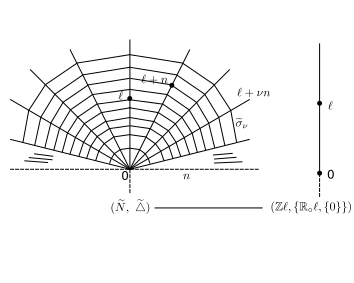
\includegraphics{vol58-fig/fig58-60.eps} 
\end{figure}
%%%%%%%
\begin{figure}[H]
\centering 
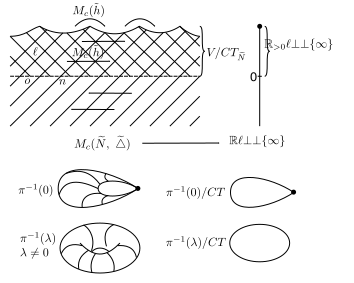
\includegraphics{vol58-fig/fig58-61.eps} 
\end{figure}\pageoriginale

\medskip
\noindent{\textbf{(2) Principally polarized 2-dimensional complex tori}}

Let $M= \mathbb{Z}^2$ with a $\mathbb{Z}-$ basis $\{m_1, m_2 \}$ and
let $N$ the dual of $M$ with the dual basis $\{n_1, n_2\}$. Then the
Delony-Voronoi decomposition of Sym$(M \times M, \mathbb{R})$ consists of the
Aut$(M)$-translates of  
$$
\sum_3 = \mathbb{R}_\circ \ell_1 + \mathbb{R}_\circ \ell_2 +
\mathbb{R}_\circ \ell_3 
$$
and its faces $\sum_2 = \mathbb{R}_\circ \ell_1 + \mathbb{R}_\circ
\ell_2 $, $\sum_1 = \mathbb{R}_\circ \ell_2 $ and $\sum_0 = {0}$, where
$\ell_1, ell_2, \ell_3 \in $ Sym $M \times M, \mathbb{Z}$ are defined as
follows: 
\begin{alignat*}{3} 
\ell_1(m_1, m_1) & = 1, \quad \ell_1(m_2, m_2) = 0, \quad  \ell_1(m_1,
m_2) &= 0,\\ 
 \ell_2(m_1, m_1) & = 0, \quad  \ell_1(m_2, m_2) = 0, \quad
 \ell_2(m_1, m_2) & = 0,\\ 
 \ell_3(m_1, m_1) & = 1, \quad  \ell_1(m_2, m_2) = 1, \quad
 \ell_3(m_1, m_2) & = -1, 
\end{alignat*}

(cf. Namikawa [{}, 2.7)]).\pageoriginale In $S^2(M)$, $\{m^2_1+m_1m_2, 
m_2^2+m_1m_2,-m_1m_2\}$ form the $\mathbb{Z}$-basis dual to $\{
\ell_1, \ell_2, \ell_3 \}$. Thus the parameter space
$\mathfrak{X}^\circ$ of 
the family of semi-universal coverings is covered by the
Aut(M)-translates of the open set isomorphic to the interior of the
closure in $\mathbb{A}_3$ of $\{( \lambda_1, \lambda_2,\break \lambda_3 )
\in \mathbb{A}_3 ; \log| \lambda_1| \log|\lambda_2|+ \log|\lambda_2|
\log|\lambda_3|+ \log|\lambda_3|\log|\lambda_1|> 0$, and $
|\lambda_1\lambda_3| <1\}$. 

We now look at semi-stable one parameter degenerations of
2 - dimensional principally polarized complex tori. It is well-known
that, up to the Aut(M)-equivalence, positive semi-definite $B \in
Sym(M \times M, \mathbb{Z})$ is of the following from:  
\begin{align*}
(1) \quad & B=0\\
(2) \quad & B(m_1, m_1)= 0,   && B(m_2, m_2) = b,   && B(m_1, m_2)= 0\\
(3) \quad & B(m_1, m_1)= a,   && B(m_2, m_2) = b,   && B(m_1, m_2)= 0\\
(4) \quad & B(m_1, m_1)= a+c, && B(m_2, m_2) = b+c, && B(m_1, m_2)= -c
 \end{align*} 
 for positive integers $a$, $b$, $c$. For simplicity, let $\tilde{h}_1=
 \tilde{h}_{m_1}$ and  $\tilde{h}_2= \tilde{h}_{m_2}$. They are the
 identity on $N_\mathbb{R}$. 
 
 In case (1), a decomposition  $\tilde{\triangle}$ satisfying our
 requirements is necessarily of the form $\tilde{\triangle}= \{\{0\},
 \mathbb{R}_o \ell\}$. 
 
 Hence $V=T \times U$ and $\pi^{-1}(0)$ is the complex torus 
 $$
 T/\{Q_0(m,?); m \in M\}.
 $$
 
 In case (2). $\tilde{h}_1(\ell)= \ell$ and $\tilde{h}_2(\ell)= \ell
 +bn_2$. For any divisor $b'$ of $b$, the decomposition of
 $\mathbb{R}n_2 + \ell$ into ``intervals''\pageoriginale of length
 $b'$ as in 
 picture below gives rise to $\tilde{\Delta}$ satisfying our
 requirements. Consider the $\mathbb{P}_1$-bundle $W$ over the
 elliptic curve $\mathbb{C}^*/ Q_0(m_1, m_1)^{\mathbb{Z}}$ obtained by
 dividing $\mathbb{C}^* \times \mathbb{P}_1$ out by the group generated by
 the automorphism $(t_1, t_2) \mapsto (Q_0(m_1,m_1)t_1, Q_0(m_1,
 m_2)t_2)$. Then by  Theorem \ref{chap1:thm4.2} (iii), we see easily that
 $\pi^{-1}(0)$ is a cycle of $b/b'$ copies of $W$ obtained by
 identifying the 0-section of one $W$ with the $\infty$-section of
 the next. If $Y$ is required to be non-singular, take $b'=1$ and get
 the Voronoi type degeneration of Namikawa and Nakamura. 
\begin{figure}[H]
\centering 
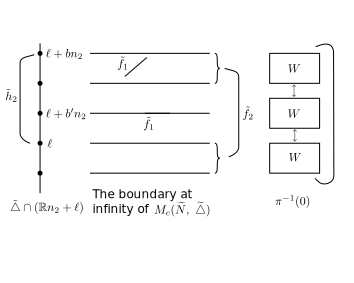
\includegraphics{vol58-fig/fig58-62.eps} 
\end{figure}
 
 In case (3), $\tilde{h}_1(\ell)= \ell + an_1$ and
 $\tilde{h}_2 (\ell)= \ell+ bn_2$.  Again for divisors $a'$ and $b'$
 of $a$ and $b$, take the decomposition of $\mathbb{R}n_1+
 \mathbb{R}n_2 + \ell$ into ``rectangles'' of size $a' \times b'$ as in the
 picture below (or a suitable sub division of it, if $Y$ is required to
 be non-singular). Without any subdivision, $\pi^{-1}(0)$ consists of
 $(a/a')(b/b')$ copies of $\mathbb{P}_1 \times \mathbb{P}_1$ glued along $0
 \times \mathbb{P}_1$, $\infty \times \mathbb{P}_1$, $\mathbb{P}_1 \times 0$,
 $\mathbb{P}_1 \times \infty$'s like a ``toroidal net'', again by Theorem
\ref{chap1:thm4.2} (iii). If  $a'= b' =1$, we\pageoriginale again get the Voronoi
type degeneration   
\begin{figure}[H]
\centering 
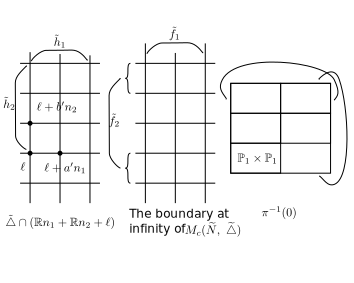
\includegraphics{vol58-fig/fig58-63.eps} 
\end{figure}
  
 In case (4), $\tilde{h}_1(\ell)= \ell +(a+c)n_1 - cn_2$ and
 $\tilde{h}_2(\ell)= \ell- cn_1 +(b+c)n_2$. There are many different
 decompositions of $\mathbb{R}n_1+\mathbb{R}n_2+ \ell$ which give rise
 to allowable $\tilde{\Delta}$'s. The ``Namikawa decompositions'' in
 Oda-Seshadri \cite{keyOS}, among which is the Voronoi type decomposition,
 are examples.  
 
 For instance, let $a= b = c = 1$, and consider the two decompositions
 below. 
 \begin{figure}[H]
\centering 
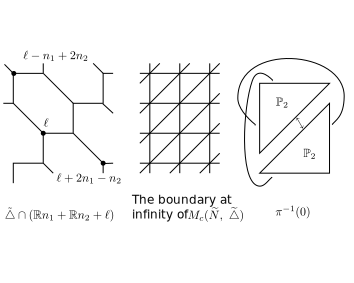
\includegraphics{vol58-fig/fig58-64.eps} 
\end{figure}
 
 It is the Voronoi type decomposition  and $\pi^{-1}(0)$ consists of
 two copies of $\mathbb{P}_2$ glued along the three coordinates axes,
 by Theorem \ref{chap1:thm4.2} (iii) and (\ref{chap1:subsec7.4}). 
 \begin{figure}[H]
\centering 
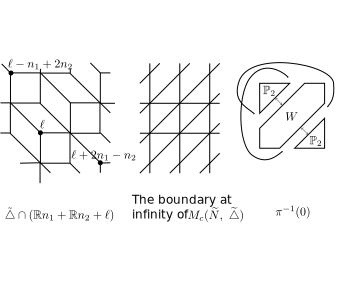
\includegraphics{vol58-fig/fig58-65.eps} 
\end{figure}\pageoriginale
 
 In this case, $\pi^{-1}(0)$ is obtained by gluing together, as in the
 picture above, two copies of $\mathbb{P}_2$ and one $W$ obtained by
 blowing $\mathbb{P}_2$ up along the three coordinates vertices,  by
 Theorem \ref{chap1:thm4.2} (iii) and Proposition
 \ref{chap1:prop6.7}. Note that $Y$ is 
 non-singular in this case and each of the six rational curves on $W$
 has the self-intersection number $-1$. This is Deligne's example
 described in Mumford \cite{keyM7}. 
 

 \section{Compact complex surfaces of class VII}\label{chap2:sec12} 
 
 Kodaira\pageoriginale \cite{keyK3} classified non-singular compact complex
 surfaces into\break seven classes. Among then, the last class $VII$ has
 been the least understood until recently.  

 \begin{defi*}
(Kodaira \cite[II, Thm 26]{keyK3}) A non-singular compact complex surface $X$
   is said to be of class $VII$ (resp. of class $VII_0$) if the first
   Betti number $b_1(X)=1$ (resp. $b_1(X) =1$ and $X$ is minimal,
   i.e. without exceptional curves of the first kind). 
 \end{defi*} 
 
 As usual, let
 \begin{gather*}
b_i(X) =\dim_{\mathbb{C}}H^i (X, \mathbb{C})\\
h^{p,q}(X) = \dim_{\mathbb{C}} H^q (\Omega^p_X)
 \end{gather*} 
 and let $c_1(x)$ and $c_2(X)$ be the Chern classes of $X$. 
 
 \noindent
 Moreover, let $b^+$ and $b^-$ be the number of positive and negative
 eigenvalues of the cup products on $H^2(X, \mathbb{R})$. 
 
 Then Kodaira \cite[I, Thm 3]{keyK3} showed that a class $VII$ surface $X$
 has the following numerical characters:  
 \begin{align*}
& h^{0,1}=1, h^{1,0}= h^{2, 0} = 0\\
& b_1 =1, b^+  = 0\\
& -c^2_1=c_2 =b_2  = b^-\\
 \end{align*} 
 
 \begin{defi*}
An, $r$-dimensional compact complex manifolds $X$ is called a {\em Hopf
  manifold} if its universal covering manifold $\tilde{X}$ is
isomorphic to $\mathbb{C}^r- \{0\}$. If, moreover,  $\pi_1 (X) \cong
\mathbb{Z}$, then $X$ is called a {\em primary} Hopf manifold. (See
e.g. \cite{keyA1} for a generalization, the Calabi-Eckmann manifold.) 
 \end{defi*} 
 
 Kodaira\pageoriginale \cite[III, Thm 41]{keyK3} gave a topological
 characterization of 2-dimensional Hopf manifolds, i.e. Hopf surfaces
 : $b_2 = 0$ and $\pi_1 (X)$ contains an infinite cyclic subgroup of
 finite index.  
 
 Again according to Kodaira \cite[II, Thm 30]{keyK3}, a primary Hopf
 surface $X$ is of the following form : 
 $$
 X =(\mathbb{C}^2-\{0\})/ \gamma^{\mathbb{Z}},
 $$
 where $\gamma^{\mathbb{Z}}$ is the group of automorphisms generated
 by $\gamma$ of the form  
 $$
 \gamma(z,z') = (\lambda z+ \mu(z')^b, \lambda' z')
 $$
 with a positive integer $b$ and $\lambda$, $\lambda'$, $\mu \in
 \mathbb{C}$ satisfying  
\begin{gather*}
 0 < | \lambda| \le |\lambda'|<1\\
 (\lambda-(\lambda')^b) \mu =0.
\end{gather*}

We have the following characterizations of some of the class $VII_0$
surfaces: 

\begin{theorem*}{\em (Kodaira [K3, II, \S. \ref{chap1:sec9} \&
      \S. \ref{chap2:sec10}])} 
 $X$ is a class $VII_0$ surface with  $b_2 = 0$ and containing at
  least one curve if and only  if $X$ is either   
\begin{itemize}
\item[a] Hopf surface, or 

\item[a] certain elliptic surface over $\mathbb{P}_1$ with at most
  non-reduced non-singular fibers, which is obtained from the product
  of $\mathbb{P}_1$ and an elliptic curve by a finite succession of
  ``logarithmic transformations''. 
\end{itemize}
\end{theorem*}

\begin{theorem*}[(Inoue \cite{keyI1})]
 $X$ is\pageoriginale a class $VII_0$ surface
with $b_2 = 0$
containing no curve, and
with a line bundle $L$ such that $H^0 (\Omega^1_X \otimes L) \neq 0$
if and only if $X$ is isomorphic to one of the surfaces  
$$
S_M, S^+_{N,p,q,r} \quad \text{and} \quad S^-_{p,q,r}
$$
constructed by Inoue.
\end{theorem*}

All these class $VII_0$ surface satisfy $b_2 = 0$. Recently, Inoue
\cite{keyI2}, \cite{keyI3} and Kato \cite{keyK2} constructed series of
example with  $b_2 
\neq 0$. As we see in \S. \ref{chap2:sec14} and \S. \ref{chap2:sec15},
these can most easily be 
described in terms of torus embeddings. 

In this connection, the following result of Kato \cite{keyK2} is of utmost
importance: 

\begin{defi*}
A \textit{global spherical shell}  in an $r$-dimensional compact complex
manifold $X$ is an open submanifold isomorphic to  
$$ 
\{ z = (z_1,\ldots, z_r) \varepsilon \mathbb{C}^r ; 1 - \varepsilon <  | z | <
1 + \varepsilon \} 
$$ 
with $0 < \varepsilon < 1$ and $|z|^2 = | z_1|^2 + \cdots + | z_r |^2$, such
that the complement in $X$ is \textit{connected}. 
 \end{defi*} 

An elliptic curve,  for instance, contains global spherical shells. 
 \begin{figure}[H]
\centering 
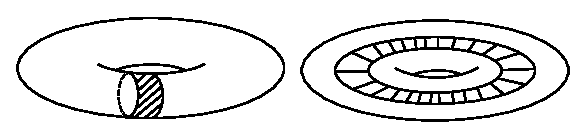
\includegraphics{vol58-fig/fig58-66.eps} 
\end{figure}

\begin{theorem*}{\em (Kato \cite{keyK2})}
 Let\pageoriginale $r \geq 2$. If an $r$-dimensional compact complex
  manifold $X$ contains a global spherical shell, then $X$ is a
  deformation of (hence is diffeomorphic to) the blowing up of a
  primary Hopf manifold along a finite number of points. In
  particular, $X$ is non-K\"ahler and $\pi_1 (X) = \mathbb{Z}$. 
\end{theorem*}

As we see in \S. \ref{chap2:sec14} and \S. \ref{chap2:sec15}, Kato
could also show that all the 
examples of Inoue with $b_2 \neq 0$ dealt  
with in \S. \ref{chap2:sec14} and \S. \ref{chap2:sec15} contain global
spherical shells, construct 
a versal family of deformations for the Inoue  
surfaces in \S. \ref{chap2:sec14} (cf. Theorem \ref{chap2:thm14.2}),
and construct may new class 
$VII_0$ surfaces with $b_2 \neq 0$ which 

contain global spherical shells (cf. Remark after Thm. 14.1).  
\

\section{Hopf surfaces and their degeneration}\label{chap2:sec13} 

In this section, we deal with those Hopf surfaces which can be
described in terms of torus embeddings. Although we restrict ourselves
to the complex case, the non-archimedean analogue might be interesting
to formulate. (cf Gerritzen-Grauert \cite{keyGG}). 

Let us first look at the primary Hopf surface
$$
X \dot{=} (\mathbb{C}^2 - \{0\}) / \gamma^{\mathbb{Z}}
$$
where $\gamma (z, z') = (\lambda z, \lambda'z')$ for $(z, z') \in
\mathbb{C}^2 - \{ 0 \}$ and $\lambda, \lambda' \varepsilon \mathbb{C}$  with
$0 < | \lambda | < 1$, $0 < | \lambda' | < 1$. 

Since $\gamma$ is defined in terms of monomials, $X$ can be described
by means\pageoriginale of torus embeddings as follows: Let $N \cong
\mathbb{Z}^2$ with a $\mathbb{Z}$-basis $\{n, n'\}$, and consider the 
r.p.p.decomposition  
$$
\triangle = \{ \mathbb{R}_o n, \mathbb{R}_o n', \{0\} \}. 
$$

Then obviously $T_N \emb (\triangle) \cong \mathbb{C}^2 - \{0 \}$,
which is simply connected for instance by Proposition
\ref{chap2:prop10.2}. $\gamma$ 
is the translation action  by $(\lambda, \lambda') = \lambda^{\langle ?, n \rangle
} {\lambda'}^{\langle ?,n' \rangle} \in T_N$. Thus it induces the
translation action 
$\bar{\gamma}$ by $ (-\log | \lambda |)\break n + (-\log | \lambda' | )n'
\in N_R $ on the manifold with corners $Mc (N, \triangle)$. As in the
picture below, the action of $\bar{\gamma}^{\mathbb{Z}}$ on $Mc (N,
\triangle)$ is properly discontinuous and fixed point free, and has a
compact fundamental domain. Thus  the action of $\gamma^{\mathbb{Z}}$
on $T_N \emb (\triangle)$ has the same properties, and we conclude
that 
$$
X = T_N \emb (\triangle) / \gamma^{\mathbb{Z}}
$$
is a non-singular compact complex surface with $\pi_1 (X) =
\mathbb{Z}$. Moreover, $X$ contains mutually disjoint elliptic curves 
\begin{gather*}
E = \orb (\mathbb{R}_o n') / \gamma^{\mathbb{Z}} \cong \mathbb{C}^* /
\lambda^{\mathbb{Z}}\\ 
E' = \orb (\mathbb{R}_o n') / \gamma^{\mathbb{Z}} \cong \mathbb{C}^* /
{\lambda'}^{\mathbb{Z}}. 
 \end{gather*} 
 
 \noindent
 By Proposition \ref{chap1:prop6.6}, the canonical bundle of $X$ is obviously 
  $$
 \omega_X = 0_X (-E-E').
 $$
  Since $E \cdot E' = 0$ and, furthermore, $E^2 = E'^2 = 0$, as we see below,
 we have $b_2 = -c_1^2 = 0 $. Indeed, the vertical  projection $N \to
 \mathbb{Z}n$ induces 
\[
\xymatrix@R=0.2cm{
\orb (\mathbb{R}_o n') \subset T_N \emb (\triangle) - \orb
(\mathbb{R}_o n) \ar[r] \ar@{}[d]^\wr|{||} & \mathbb{C}^*  \\
\mathbb{C}^* \times \mathbb{C} &  
}
\]
on which\pageoriginale $\gamma$ acts by $\gamma (z, z') = (\lambda z,
\lambda' z')$. Dividing these out by $\lambda^{\mathbb{Z}}$, we get  
$$
E \subset X - E \longrightarrow \mathbb{C}^*  / \lambda^{\mathbb{Z}}. 
$$
$X-E'$ is obviously the total space $V(L)$ of a line bundle $L$ of
degree 0 on the elliptic curve $\mathbb{C}^*/  \lambda^{\mathbb{Z}}$
and $E$ is its 0-section. Thus 
$$
E^2 = -\deg L = 0 .
$$
$X$ is thus a rather curious compactification of $V(L)$.


$X$ has a global spherical shell indicated in the picture.
 \begin{figure}[H]
\centering 
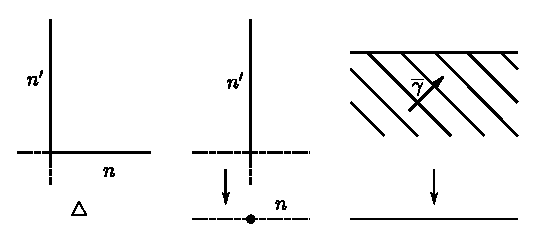
\includegraphics{vol58-fig/fig58-67.eps} 
\end{figure}
%%%
 \begin{figure}[H]
\centering 
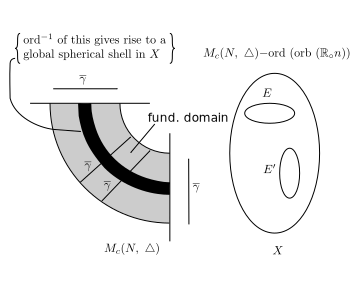
\includegraphics{vol58-fig/fig58-68.eps} 
\end{figure}

For\pageoriginale a positive integer a, let $\bar{F}_a$ be the
non-projective algebraic surface with an ordinary double curve
obtained by identifying the 0-section and the $\infty$-section  of
the rational ruled surface  
$$
F_a = \mathbb{P} (0_{\mathbb{P}_1} \otimes 0_{\mathbb{P}_1} (a)) 
$$
by means of the map $(z, 0) \mapsto (\phi (z), \infty)$ for $\phi
\in$  Aut  $(\mathbb{P}_1)$. Assuming that the coefficients of $\phi$
as a linear fractional transformation are small, Kodaira \cite[III,
  Thm 45]{keyK3} showed: 

\begin{theorem*}
There exists a complex analytic family over the unit disk 
$$
\pi (a) : Y (a) \longrightarrow U = \{ \lambda \in \mathbb{C} ; |
\lambda | < 1 \} 
$$
such that 
$$
\pi (a) ^{-1}(0) = \bar{F}_a   
$$
and $\pi(a)^{-1}_{(\lambda)}$ is a Hopf surface for $\lambda \neq 
0$. 
\end{theorem*}

Using torus embeddings, we prove this theorem in the special case
where $\phi$ is the identity. The proof can be modified so that it
works for $\phi (z) = cz^{\pm}$, $c \in \mathbb{C}^*$. 

For this purpose, let us first consider the following Hopf surface: As 
before, let $N \cong \mathbb{Z}^2$ with a basis $\{ n, n'\}$. For a
positive integer a, let 
$$
\triangle (a) = \{\mathbb{R}_o n, \mathbb{R}_o (-n + an'), \{0 \} \}. 
$$ 

\noindent
Then by Proposition \ref{chap2:prop10.2}, we see that 
$$
\pi_1 (T_N \emb (\triangle (a)) \cong \mathbb{Z} / a \mathbb{Z}.
$$
In\pageoriginale fact the universal covering space is $T_{N'} \emb
(\triangle (a)) \cong \mathbb{C}^{2}  - \{0\}$, where $N' \subset N$
is the subgroup generated by  $n$ and $-n + an'$. By
(\ref{chap1:subsec7.6'}$'$), we also 
see that $T_{N}\emb(\triangle(a))$  is the complement of the
0-section and the $\infty$-section of $F_{a}$.   

For $\lambda$ in the punctured unit disk $U^{*}$, consider the
translation action $\gamma_{\lambda}$ on $T_{N}\emb(\triangle(a))$ of  
$$
\lambda^{< ?, n'>}\in T_{N}. 
$$ 

Then the induced action $\bar{\gamma}_{\lambda}$ on $Mc (N,
\triangle(a))$ is the translation by $(-\log | \lambda |) n'$, hence
is properly discontinuous, fixed point free with a compact fundamental
domain.   

Thus we see that 
$$
X_{\lambda}(a) = T_{N} \emb (\triangle(a)) / \gamma^\mathbb{Z}_{\lambda}
$$
is a Hopf surface with 
$$
\pi_{1}(X_{\lambda}(a)) \cong \mathbb{Z}~ x~ \mathbb{Z}/
a\mathbb{Z}.
$$
 \begin{figure}[H]
\centering 
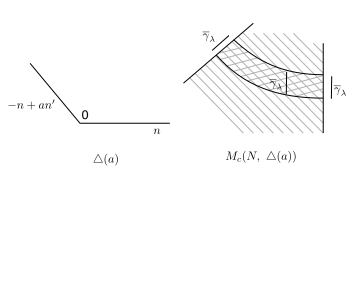
\includegraphics{vol58-fig/fig58-69.eps} 
\end{figure}

We then consider $\tilde{N} = N \oplus \mathbb{Z} \ell$ and its
automorphism $\tilde{\gamma}$ defined by  
$$
\tilde{h}(n) = n, \quad \tilde{h}(n') = n' ,  \quad \tilde{h} (\ell) =
\ell + n'. 
$$

Let\pageoriginale $(\tilde{N}, \tilde{\triangle}(a))$ be the
r.p.p.decomposition consisting of the faces of $\sigma_{\nu}$,
$\sigma'_{\nu}$ with $\nu$ running through $\mathbb{Z}$, where  
\begin{align*}
\sigma_{\nu} & = \mathbb{R}_{o}n + \mathbb{R}_{o} (\ell + \nu n') +
\mathbb{R}_{o} (\ell + (\nu - 1) n')\\ 
\sigma'_{\nu} & =  \mathbb{R}_{o} (-n + an') +  \mathbb{R}_{o} (\ell +
\nu n') + \mathbb{R}_{o} (\ell + (\nu - 1) n'). 
\end{align*}
 
\noindent 
Thus $\tilde{\triangle}(a) \cap N_{\mathbb{R}} = \triangle (a)$ and
$\tilde{\triangle}(a)$ induces on the affine subspace $N_{\mathbb{R}}
+ \ell$ the polyhedral decomposition $\tilde{\triangle}(a) \cap
(N_{\mathbb{R}} + \ell)$ as in the picture below. $\tilde{h}$
preserves $\tilde{\triangle}(a)$ and gives rise to an automorphism
$\bar{\gamma}$ of non-singular $T_{\tilde{N}} \emb
(\tilde{\triangle}(a))$.  
 
\noindent
Note that the boundary at infinity of $Mc (\tilde{N}, \tilde{\triangle
}(a))$ consists of two ``walls'' $\orb (\mathbb{R}_{o}n) /
CT_{\tilde{N}}$ and $\orb (\mathbb{R}_{o} (-n +  an')) /
CT_{\tilde{N}}$  as well as the ``roof'' as in the picture.    
 
The horizontal projection induces 
$$
\tilde{\pi}(a) : T_{\tilde{N}} \emb (\tilde{\triangle} (a)) \to
T_{\mathbb{Z} \ell} (\{ \mathbb{R}_{o}\ell, \{0\} \}) = \mathbb{C}. 
$$ 
 
\noindent
Let $V$ be the inverse image of the unit disk $U$ by $\tilde{\pi}(a)$.  
 
\noindent
Thus $\ord (V)$ is the upper half of $Mc (\tilde{N},
\tilde{\triangle}(a))$.  
 
The action of $\bar{\gamma}^{\mathbb{Z}}$ on $V$ is properly
discontinuous and fixed point free, $\tilde{\gamma}$ coincides with
$\gamma_{\lambda}$ above on $\tilde{\pi}(a)^{-1}(\lambda) = T_{N}
\emb (\triangle (a)) x \{\lambda\}$. Hence  
$$
\pi (a) : Y (a) = V/ \tilde{\gamma}^{\mathbb{Z}} \to U 
$$
is the sougth-for family with 
$$
 \pi (a)^{-1} (0) = \bar{F}_{a}~ \text{ and }~ \pi (a)^{-1} (\lambda) 
 = X_{\lambda}(a) ~\text{ for }~ \lambda \neq 0 
$$
by Theorem \ref{chap1:thm4.2} (iii) and (\ref{chap1:subsec7.6'}$'$). 
 \begin{figure}[H]
\centering 
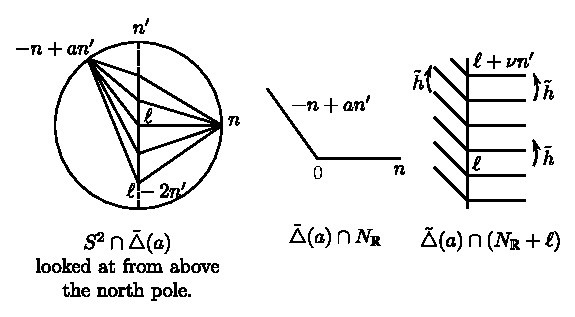
\includegraphics{vol58-fig/fig58-70.eps} 
\end{figure}
%%%%
 \begin{figure}[H]
\centering 
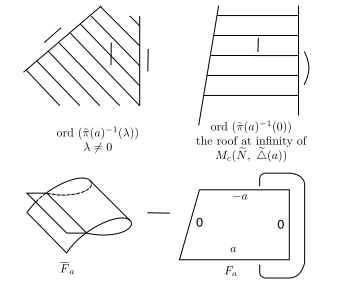
\includegraphics{vol58-fig/fig58-71.eps} 
\end{figure}\pageoriginale

\section[Inoue's examples of class $VII_{0}$ surfaces...]{Inoue's examples 
of class $VII_{0}$ surfaces with \break $b_{2} = 1$}\label{chap2:sec14} 
  
Torus embeddings are very convenient to describe Inoue's examples of
class $VII_{0}$ surfaces with $b_{2} \neq 0$. In this section we
describe the first series of his examples in \cite{keyI2}. Besides, we will
be able to describe their degeneration easily in terms of torus
embeddings. We also sketch Kato's generalization of
Inoue's\pageoriginale construction which provides us with many new
examples.   
  
As before, let $N \cong \mathbb{Z}^{2}$ with a basis $\{n, n'
\}$. Consider the r.p.p. decomposition $(N, \triangle)$, where  
\begin{gather*}
\triangle = \{\mathbb{R}_{o}n' ~\text{ and the faces of }~ \sigma_{\nu}
~\text{for }~ \nu \in \mathbb{Z}\}\\ 
\sigma_{\nu} = \mathbb{R}_{o}(n + \nu n') + \mathbb{R}_{o} (n + (\nu -
1) n').  
\end{gather*}  
 By Proposition \ref{chap2:prop10.2}, $T_{N} \emb (\triangle)$ is
 simply connected. Let 
$h$ be the automorphism of $N$ defined by  
$$
h (n) = n + n', \quad  h (n') = n'. 
$$
$h$ obviously preserves $\triangle$ and gives rise to the automorphism
$h_{*}$ of $T_{N}\break \emb (\triangle)$.  
  
For $\lambda \in U^{*} =\{\lambda \in \mathbb{C} ; 0 < | \lambda | <
1\}$, consider the automorphism   
$$
\gamma_{\lambda} = ~ (\text{the translation by }~ \lambda^{\langle ? ,
  n \rangle} ) \circ h_{*} 
$$
of $T_{n}\emb (\triangle)$. For $(z, z') \in T_{N}$, we see that 
$$
\gamma_{\lambda} (z, z') = (\lambda z , zz'),   
$$
hence 
$$
\gamma_{\lambda}^{\nu} (z , z') = (\lambda^{\nu} z , \lambda^{\nu
  (\nu-1)/2} z^{\nu} z')~ \text{ for }~  \nu \in \mathbb{Z}. 
$$ 
$\gamma_{\lambda}$ induces an automorphism $\bar{\gamma}_{\lambda}$ of
$Mc (N, \triangle)$
$$
\bar{\gamma}_{\lambda} = (\text{the translation by }~ (-\log | \lambda
|)n) \circ Mc (h) .  
$$
  
As we see easily in the picture, the action of
$\bar{\gamma}^{\mathbb{Z}}_{\lambda}$, hence that of
$\gamma^{\mathbb{Z}}_{\lambda}$, is properly discontinuous, fixed
point free and with a compact fundamental domain. Thus  
$$
X_{\lambda} = T_{N} \emb (\triangle) / \gamma^{\mathbb{Z}}_{\lambda} 
$$
is a non-singular compact complex surface with $\pi_{1} (X_{\lambda}) 
= \mathbb{Z}$, in\pageoriginale particular $b_{1} = 1$. 
 \begin{figure}[H]
\centering 
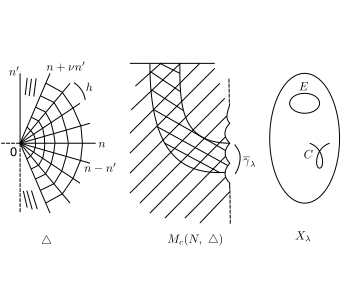
\includegraphics{vol58-fig/fig58-72.eps} 
\end{figure}

\begin{theorem}[Inoue \cite{keyI2}]\label{chap2:thm14.1}
 For $\lambda  \in U^{*}$, the surface $X_{\lambda}$ is
  of class $VII_{0}$ with $b_{2} = 1 \cdot X_{\lambda}$ has exactly two
  irreducible curves, an elliptic curve $E$ and a rational curve $C$
  with a node, such that   

$E^{2} = -1$,  $C^{2} = 0$, $E \cdot C = 0$ and $C$ homologous to zero

$H^{2} (X_{\lambda}, \mathbb{Q})$ is 1-dimensional and is generated by
  $E$. 
\end{theorem}

\begin{proof}
$\orb (\mathbb{R}_{o} n') = \mathbb{C}^{*}$ is certainly
  $\gamma^{\mathbb{Z}}_{\lambda}$-invariant and $E =
  \orb(\mathbb{R}_{o} n') / \gamma^{\mathbb{Z}}_{\lambda}  \cong
  \mathbb{C}^{*}/ \lambda^{\mathbb{Z}}$ is an elliptic curve. On the
  other hand, the closure of $\orb (\mathbb{R}_{o} (n + \nu n')$
 is $\mathbb{P}_{1}$ for $\nu \in \mathbb{Z}$, and
  their union $C^{*}$ is
  $\gamma^{\mathbb{Z}}_{\lambda}$-invariant. $C = C^{*}/
  \gamma^{\mathbb{Z}}_{\lambda}$ is a 
  rational curve obtained from $\mathbb{P}_{1}$ by identifying 0 and
  $\infty$. Since $\mathbb{C}^{*}$ is the fiber of the equivariant
  morphism 
$$
T_{N} \emb (\triangle) \longrightarrow  T_{\mathbb{Z}n} \emb 
(\{\mathbb{R}_{o}n, \{0\}\}) 
$$
induced by the vertical projection, we see that  $C^{2} = 0$. 
Certainly, $C$ and $E$ are disjoint, hence $C \cdot E = 0$. Let us
now\pageoriginale look at    
\[
\xymatrix@R=0.4cm{
\orb(\mathbb{R}_{o}n') \subset T_{N}\emb (\{\mathbb{R}_{o}n', \{0\}
\}) \ar[r]  \ar@{}[d]|{||}&  T_{\mathbb{Z}n} \emb (\{0\}) =
\mathbb{C}^{*}   \\ 
\mathbb{C}^\ast \times \mathbb{C}
}
\]
on which $\gamma^{\mathbb{Z}}_{\lambda}$ acts via
$\gamma^{\nu}_{\lambda} (z, z') = (\lambda^{\nu} z, \lambda^{\nu
  (\nu-1)/2} z^{\nu} z')$.  
Dividing these out, we have 
$$
E \subset X_{\lambda} - C \longrightarrow \mathbb{C}^{*}/
\lambda^{\mathbb{Z}},   
$$
which makes $X_{\lambda} - C$ the total space $V(L)$ of a line bundle
$L$ of degree 1 over $\mathbb{C}^{*} / \lambda^{\mathbb{Z}}$ and $E$
its 0-section. Hence $E^{2} = -\deg L = -1$. 

\noindent
By Proposition \ref{chap1:prop6.6}, we see that the canonical bundle is  
$$
\omega_{X_{\lambda}} = 0_{X_{\lambda}} (-E - C),  
$$
hence $b_{2} = -c^{2}_{1} = - (-E - C)^{2} = 1$. Thus $H^{2}
(X_{\lambda}, \mathbb{Q})$ is necessarily spanned by $E$ and $C$ is
homologous  to zero.  
\end{proof}

Suppose there were an irreducible curve $D \neq E, C$. 

\noindent
Since $C  \cdot D = 0$, $D$ would be contained in $X_{\lambda} - C =
V(L)$. Thus $E \cdot D$, which is non-negative by assumption, would be the
degree of the pull-back of $L^{-1}$ by $D \to V(L) \to \mathbb{C}^{*}
/ \lambda^{\mathbb{Z}}$, a contradiction. $X_{\lambda}$ is minimal,
since it thus has no exceptional curve of the first kind.  

\begin{remark*}
Kato \cite{keyK2} looks at $X_{\lambda}$ this way: it is obtained, from
$\ord^{-1}$ of the shaded area in $Mc(N, \triangle)$, by identifying
via $\gamma_\lambda$ the\pageoriginale two spherical shells which is
$\ord^{-1}$ of the two thick arcs in the picture.     
 \begin{figure}[H]
\centering 
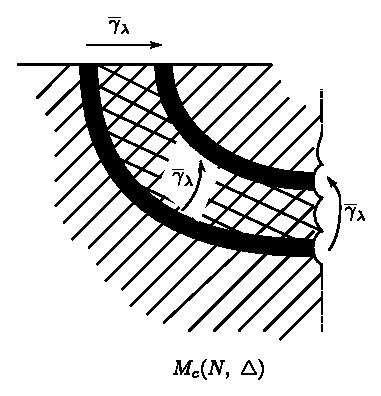
\includegraphics{vol58-fig/fig58-73.eps} 
\end{figure}
\end{remark*}
 
In this way, we need to consider not $T_N \emb (\Delta)$ but the
simpler torus  embedding 	 
$$
Z= T_N \emb(\{\mathbb{R}_\circ n, \mathbb{R}_\circ (n+n'),
\mathbb{R}_\circ n', \{0\}\}  
$$ 
obt ained by  blowing up $\mathbb{C}^2$ along 0.  Hence $Z=V_1 \cup
V_2$ with $V_1 =\mathbb{C}^2$ and $ V_2 =\mathbb{C}^2$  with
coordinates $(z, \zeta)$ and $(z' ,\zeta')$, respectively, glued along
$(\mathbb{C}^*)^2$  via  
    $$
    z'=z \zeta \text{ and } \zeta' = \zeta^{-1}.
    $$
    
    Let $\phi_\lambda : \mathbb{C}^2 \to V_1 \subset Z$be defined by 
    $$
    \phi_\lambda (z, z')= (\lambda z, z' / \lambda).
    $$
    
    Consider, for $\varepsilon > 0$ small, the spherical shell 
    $$
    \sum= \{ (z, z' ) \in  \mathbb{C} ^2  ; 1 - \varepsilon<
    (|z|^2 + |z'|^2)^{1/2}< 1 + \varepsilon\} 
    $$ 
   and its inverse image $\sum'$ by the blowing up $z \rightarrow
   \mathbb{C}^2$. Let $\sum_\lambda'' = \phi_\lambda (\sum)$. Then
   $\sum'$ and $\sum_\lambda''$ are 
   spherical shells whose images under ord are the thick arcs in the
   picture. Thus $\phi_\lambda$ induces an isomorphism $ \psi_\lambda
   : \sum' \xrightarrow{\sim} \sum_\lambda''$.  
   \begin{figure}[H]
\centering 
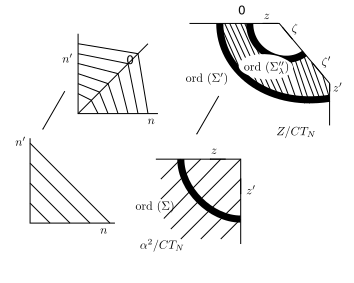
\includegraphics{vol58-fig/fig58-74.eps} 
\end{figure}
   
   Then\pageoriginale $X_\lambda$ is obtained from the inverse image
   in $Z$ of the shaded area between the thick arcs $\ord (\sum')$ and $\ord
   (\sum''_{\lambda})$ by identifying $\sum'$ and $\sum_{\lambda''} 
   $ via $\psi_\lambda$. The common image of $\sum'$ and
   $\sum''_\lambda$ in $X_\lambda$ is obviously a global spherical
   shell.     
   
   This process was generalized by Kato \cite{keyK2}  to produce new class
   $VII_0$ surfaces with global spherical shells. Instead of $Z$, he
   takes $Z'$ obtained from  $\mathbb{C}^2$  by a finite
   succession of blowing ups each time along a point over the previous
   center. 
   
   Kato's formulation also enabled him to construct a versal family of
   deformations of Inoue's example $X_\lambda$. As before, let $U^*$
   be the punctured unit disk and let $B \subset \mathbb{C}^2 $
 be a small open ball centered at 0 with the coordinate
   $(\tau, \tau')$.  
   
   \begin{theorem}[Kato \cite{keyK2}]\label{chap2:thm14.2}
There exists a versal family of deformations 
$$
\mathscr{X}=\{ X_{ \lambda, \tau, \tau' }; ( \lambda , \tau , \tau')
  \in U^* \times B\} \longrightarrow U^* \times B  
$$
and families of curves
$$
\mathscr{C} = \{ C_{\lambda, \tau , \tau'}\} \quad \text{and} \quad 
\mathscr{E} = \{E_{\lambda, \tau, \tau'}\}  
$$
 in $\mathscr{X}$ such that 
 \begin{enumerate}[(i)]
\item  $X_{\lambda, 0, 0}= X_\lambda$ is Inoue's  example with
  $C_{\lambda, 0,0} = C$ and $ E_{ \lambda , 0,0}=E$ of Theorem
  \ref{chap2:thm14.1}. 

\item For $\tau '  \neq 0$, $E_{\lambda, 0, \tau '}$ is empty and
  $X_{\lambda, 0, \tau '}$ is a new class $VII_0$ surface with a
  unique irreducible curve $C_{ \lambda, 0, \tau'}$ rational with a
  node of self-intersection number 0.  

For\pageoriginale different $ \tau ' \neq 0  's ,  X_ { \lambda, 0
  ,\tau'}$  are all isomorphic.   

\item For $\tau  \neq 0$, \quad  $X_{\lambda, \tau, \tau'}$ is blowing
  up of a primary Hopf surface  along a point. 
 \end{enumerate} 
   \end{theorem}   
   
   Here is a sketch of the construction: Let $Z=V_1 \cup V_2$ and
   $\sum'$ be as in the Remark above. Consider  
     $$
   \phi_{\lambda , \tau , \tau'}: \mathbb{C}^2 \longrightarrow V_1
   \subset Z 
   $$
   \noindent
   defined by $\phi_{ \lambda, \tau,\tau'}(z, z') = ( \lambda(z_
   \tau), ( z \zeta + \tau ' ) / \lambda)$. 
   
   \noindent
   It again induces an isomorphism
   $$
   \psi_{\lambda, \tau, \tau '}: \sum ' \tilde{\longrightarrow} 
   \sum''_{\lambda, \tau , \tau '}= \phi_{\lambda, \tau, \tau
     '}(\sum '). 
   $$ 
   
   \noindent
   Then take $\ord^{-1}$ of the shaded area in the picture of $Z/CT_N$.
   Let $X_{\lambda, \tau, \tau ' }$ be the manifold obtained from it
   by   identifying $ \sum '$ and $\sum_{\lambda,\tau,\tau'}
   \text{via } \psi_{ \lambda, \tau, \tau '}$.  We then let $\mathscr{C}$ and
   $\mathscr{E}$  be the images in $\mathscr{X}$ of  
   $$
   \{ ( z' , \zeta' , \lambda, \tau , \tau') \in V_2 \times U^* \times B : z'
   \zeta ' + \lambda ' + \lambda \tau/ (\lambda-1) =0\}
$$
 and
$$
 \{ (z, \zeta' , \lambda, \tau, \tau ') \in V_1 \times U^* \times B ; \zeta
   =\tau ' =0\}, 
$$
respectively.
\begin{figure}[H]
\centering 
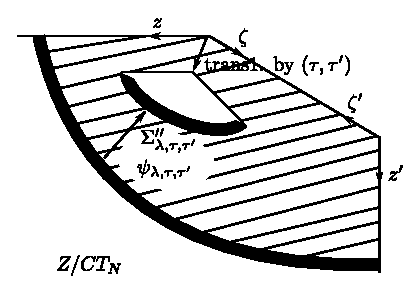
\includegraphics{vol58-fig/fig58-75.eps} 
\end{figure}
%%%
\begin{figure}[H]
\centering 
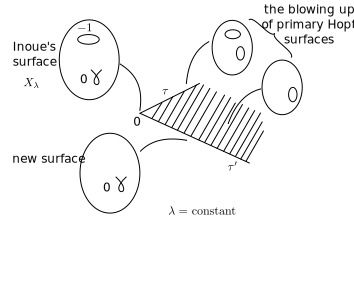
\includegraphics{vol58-fig/fig58-76.eps} 
\end{figure}\pageoriginale
   
We now look at the   degeneration of Inoue's surface $X_\lambda$ as
$\lambda$ tends to 0. 

\begin{theorem}\label{chap2:thm14.3}%% 14.3
There exists a proper flat family
$$
\Pi : \lambda \longrightarrow U = \{ \lambda \in
\mathbb{C}  ; | \lambda | < 1\} 
$$
with $Y$ non-singular such that for $\lambda \neq 0$ \;\;
$\Pi^{-1}(\lambda)$ is Inoue's surface $X_\lambda$, and that
$\Pi^{-1}(0)$ is a non-normal surface obtained by identifying two 
$\varmathbb{P}_1 's$ on the 2-dimensional complete non-singular
torus embedding $W$  as in the picture. 
\begin{figure}[H]
\centering 
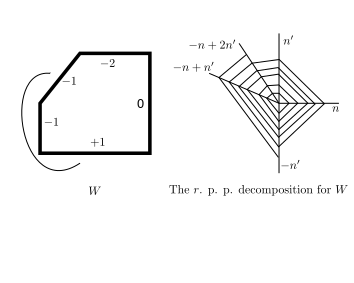
\includegraphics{vol58-fig/fig58-77.eps} 
\end{figure}
\end{theorem}

\begin{proof}
 Let $\widetilde{N}= N \otimes \varmathbb{Z} \ell$ and consider 
 the automorphism $\widetilde{h}$ of $\widetilde{N} $ defined by 
 $$
 \widetilde{h}(n) =n + n', \quad  \widetilde{h}(n'), \quad
 \widetilde{h}(\ell)  = \ell +n .  
$$
  Let ($\widetilde{N}, \; \widetilde{\Delta}$) be the 
  r.p.p.decomposition, where $\widetilde{\Delta}$ consists of
  the\pageoriginale   faces of   
  \begin{align*}
 & \varmathbb{R}_o\widetilde {h} ^ \nu(\ell) +   \varmathbb{R}_o\widetilde
    {h} ^ {\nu+1}(\ell) +\varmathbb{R}_o\widetilde {h}^{\nu-1}(n)\\ 
    &\varmathbb{R}_o\widetilde {h} ^ {\nu +1}(\ell) +
    \varmathbb{R}_o\widetilde {h} ^ {\nu -1}(n) +
    \varmathbb{R}_o\widetilde {h} ^ \nu(n)\\ 
      &\varmathbb{R}_o\widetilde {h} ^ \nu(\ell) +
    \varmathbb{R}_o\widetilde {h} ^ {\nu +1} (\ell ) +
    \varmathbb{R}_on' 
 \end{align*}
 with  $\nu$ running through $\varmathbb{Z}$. Then $
 \widetilde{\Delta} \cap N_{\varmathbb{R}}$ coincides with $\Delta$
 of  Theorem \ref{chap2:thm14.1},  and $\widetilde{\Delta}$ inducers the
 polyhedral  decomposition $\widetilde{\Delta} \cap (N_{\varmathbb{R}}
 + \ell )$  as  in the picture below. Note that   
 $$
 \widetilde{h}^\nu(\ell) =\ell + \nu n + ( \nu (\nu -1) /2 ) n'.
 $$
 Obviously, $\widetilde{h}$ preserves $\widetilde{\Delta}$ and gives
 rise to an automorphism $\widetilde{\gamma}$ of $
 T_{\widetilde{N}}\break\emb (\widetilde{\Delta})$. The horizontal
 projection induces $\widetilde{\Pi}: T_{\widetilde{N}}\emb
 (\widetilde{\Delta}) \longrightarrow T_{\varmathbb{Z}\ell}\break \emb (\{
 \varmathbb{R}_o \ell , \{0\}\})= \mathbb{C}$. Again let $V$ be
 the inverse image of the unit disk $U$  under $\widetilde{\pi}$. Thus
 ord (V) is the ``upper half'' of
 $Mc(\widetilde{N},\widetilde{\Delta})$. The action of 
 $\widetilde{\gamma}^{\varmathbb{Z}}$ on $V$   is properly
 discontinuous and fixed point free. Again by Theorem
 \ref{chap1:thm4.2} (iii) and  Proposition \ref{chap1:prop6.7}, we see that  
  $$
 \pi : Y = V/\widetilde{\gamma}^{\varmathbb{Z}} \longrightarrow U 
 $$
  is the sought-for family
\begin{figure}[H]
\centering 
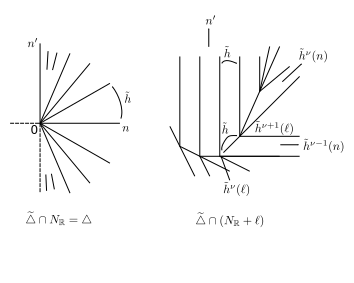
\includegraphics{vol58-fig/fig58-78.eps} 
\end{figure}
%%% 
\begin{figure}[H]
\centering 
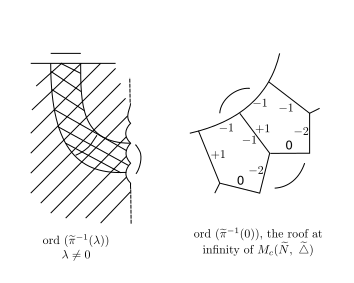
\includegraphics{vol58-fig/fig58-79.eps} 
\end{figure}
\end{proof}\pageoriginale


  \section{Hilbert modular surfaces and class $VII_0$
    surfaces}\label{chap2:sec15}  
  
   Inoue \cite{keyI3} constructed another series of examples of class
   $VII_0$ surfaces with  $b_2 \neq 0$, using the minimal
   desingularization by  Hirzebruch \cite{keyH4} of neighborhoods of cusps
   of the Hilbert modular surfaces. Again torus embeddings are very
   convenient to describe them.  
   
   We first describe the relevant part of Hirzebruch's  theory in
   terms of torus embeddings. (See also Cohn \cite{keyC2}.) For  the
   complete description of compactified Hilbert modular surfaces, we
   refer the reader to Mumford et al. \cite[Chap. \ref{chap1},
     \S. \ref{chap1:sec5}]{keySC}. See 
   also Rapoport \cite{keyR1} for the case of totally  real fields in
   general.  
   
  Let\pageoriginale $K= \mathbb{Q}(\sqrt{d})$  be a real quadratic
  field. Then  we have two embeddings of $K$ into $\varmathbb{R}$   
    $$
   K\ni \xi \mapsto \xi  \in \varmathbb{R} \quad \text{and} \quad
   K\ni \xi \mapsto \xi' \in \varmathbb{R}  
  $$
    so that we have a canonical isomorphism of
    $\varmathbb{R}$-algebras  
  $$
    \varmathbb{R} \otimes_{\mathbb{Q}} K \ni a \otimes \xi \mapsto (a
    \xi, a \xi ') \in   \varmathbb{R}^2 
  $$
    with which we identify them from now on.
  
  \begin{defi*}
 For a $\varmathbb{Z}-$lattice $N$ in $K$, let  
  \begin{align*}
U_N &= \{ \text{positive units $u$ of $k$ such that } u_N=N\}\\ 
U_N^+ &= \{\text{totally positive units $u$ of $k$ such that } uN=N\}.
 \end{align*} 
  \end{defi*}  

  Then it is known (see, for instance Hirzebruch \cite{keyH4}) that  $U_N$
  and $U_N^+$ are \textit{infinite cyclic groups} with  
    $$
  [U_N  : U_N^+] = 1 \text{ or }   2.
  $$

  We have the canonical identification
    $$
  N_{\varmathbb{R}}=  \varmathbb{R} \otimes_{\mathbb{Q}} K = \varmathbb{R}^2
   $$
    with $N$ lying irrationally in $\varmathbb{R}^2$ with respect to
    the coordinate system of $\mathbb{R}^2$. Consider the convex hull
    $\sum_N '$  of  
    $$
 N \cap (\varmathbb{R}_{>0})^2  
  $$
    and the infinite r.p.p.decomposition $(N, \Delta_N ')$, where
  $\Delta_N'$ is the decomposition of the first quadrant $(
  \varmathbb{R}_{>0})^2$ into sectors by rays joining 0 and the
  points in $N \cap \partial \sum_N '$. 
  
  Thus $ Mc(N, \Delta_N ')$  is the union of $N_{\varmathbb{R}} $and
  the infinite chain of intervals at infinity. 

The\pageoriginale action of $U^+_N$ on $N$ by multiplication certainly
preserves $\Delta'_N$, hence we have an action of $U^+_N$ on $T_N
\emb(\Delta'_N)$.  Let $V'_N$ be $\ord^{-1}$ of the union of the first
quadrant $(\mathbb{R}_{> 0})^2$ and the boundary at infinity of $Mc (N, 
\Delta'_N)$. Then the action of $U^+_N$ on $\ord (V'_N)$, hence that
on $V'_N$ itself, is properly discontinuous and fixed point free.
Thus the quotient   
$$
W'_N = V'_N/ U^+_N
$$
(or, more generally,  the quotient by a subgroup of $ U^+_N$ of finite
index) is non-singular,  and contains a finite cycle of
$\mathbb{P}_1 's$.  Such $W'_N$ appears as a neighborhood of the
minimal resolution of a cusp of a Hilbert modular surface. 
\begin{figure}[H]
\centering 
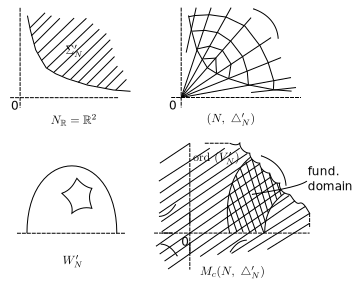
\includegraphics{vol58-fig/fig58-80.eps} 
\end{figure}

Inoue\pageoriginale \cite{keyI3} obtains a new class $VII_0$ surface by
gluing two appropriate such $W'_N$'s together. In our formulation,
this amounts to applying the process above to the first and the fourth
quadrant simultaneously:  

\begin{theorem}[Inoue]\label{chap2:thm15.1}
 Let $N$ be a $\mathbb{Z}$-lattice in a real quadratic
  field $K$.  Let $\sum'_N$ (resp. $\sum''_N$) be the convex hull of $N
  \cap (\mathbb{R}_{>0})^{2}$ (resp. $N \cap (\mathbb{R}_{>0} \times
  \mathbb{R}_{<0}))$. Consider the infinite r.p.p.decomposition
  $(N, \Delta_N)$, where $\Delta_N$ is the decomposition of
  $\mathbb{R}_{>0} \times \mathbb{R}$ into sectors by rays joining 0 and  
$$ 
(N \cap \partial \sum'_N)  \cup (N \cap \partial \sum''_N). 
$$
Let $V_N$ be $\ord^{-1}$ of the union of $\mathbb{R}_{>0} \times \mathbb{R}$
and the boundary at infinity of $Mc(N,\triangle_N)$. Then the
following hold:  
\begin{enumerate}[(i)]
\item \qquad $X_N = V_N/ U^+_N$ is a non-singular compact surface of
  class $VII_0$ with exactly $b_2 \neq 0$ irreducible curves, which
  form two disjoint cycles of rational curves.  

\item If $[U_N : U^+_N] = 2$, then 
$$
\hat{X}_N = V_N/ U_N
$$
is also a non-singular compact complex surface of class $VII_0$ with
exactly. $b_2 \neq 0$ irreducible curves, which form a cycle of
rational curves.  
\end{enumerate}
\end{theorem}

Here is a sketch of the proof: 

From\pageoriginale the picture below, the action of $U^+_N$ (or $U_N$
in case $(ii)$) 
on $V_N$ is easily seen to be properly discontinuous, fixed point free
and with a compact fundamental domain. 

Note that in case $(ii)$, the multiplication by an element of $U_N$
not in $U^+_N$ interchanges the first and the fourth quadrant, hence
$\Delta_N$ is in a sense ``symmetric''.  

$\ord^{-1}$ of the two infinite chains of the boundary gives rise to 
two disjoint cycles  
\begin{align*}
C & = C_0+ C_1 + \cdots + C_{r-1} \\
C & = D_0+ D_1 + \cdots + D_{r-1}
\end{align*}
of rational curves in $X_N$. In case $(ii)$, we have $ r = s $ and the
images of $C$ and $D$ in $\hat{X}_N$ coincide. We thus have a cycle of
rational curves  
$$
\hat{C}= \hat{C}_0 + \hat{C}_1 + \cdots \hat{C}_{r-1} 
$$
\begin{figure}[H]
\centering 
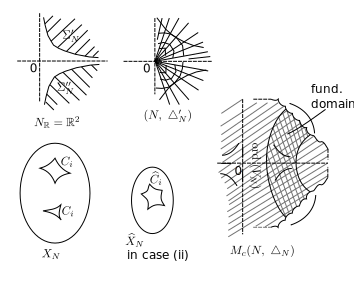
\includegraphics{vol58-fig/fig58-81.eps} 
\end{figure}

We refer\pageoriginale reader to Inoue \cite{keyI3} for the proof of the
facts:  
\begin{align*}
 H_1(X_N, \mathbb{Z}) & \cong \mathbb{Z}\\
 H_2(X_N, \mathbb{Z}) & \cong \mathbb{Z}^{\oplus (r+s)}
\end{align*}
$C_0, \ldots , C_{r-1}$ and $D_0, \ldots , D_{s-1}$ are the only
irreducible curves in $X_N$. In particular, $X_N$ and $\hat{X}_N$ are
minimal. 
Note that from the picture, we easily see that $\ord^{-1}$ of the
positive half of the abscissa in $Mc(N, \Delta_N)$ gives rise to a
$CT_N$-bundle over $S^1$ in $X_N$, and that $X_N -C-D$ is homeomorphic
to the product of $\mathbb{R}$ and the bundle. 

\begin{remark*}
As Kato \cite{keyK2} has shown, $X_N$ contains a global spherical shell,
hence is deformation of the blowing up of a primary Hopf surface along
a finite number of points. Indeed, $\ord^{-1}$ of a tubular
neighborhood of the boundary of our fundamental domain in the picture
gives rise to one 
\end{remark*}

To study $W'_N$, $X_N$ and $\hat{X}_N$ in more detail, the ``modified''
continued fraction expansion is very convenient as in Hirzebruch
\cite{keyH4} and Inoue\cite{keyI3}. 

\begin{defi*}
Let $\xi$ be a real number. Then the modified continued fraction
expansion 
$$
\xi = [[ e_0,e_1 , \ldots]]
$$
is defined as follows:  For non-negative integers $\nu$ determine 
$\xi_{\nu}$ and $e_{\nu}$ inductively by  
\begin{align*}
& \xi_0 = \xi \\
& e_{\nu} \quad \text{ is the integer with } e_{\nu} - 1 < \xi_{\nu}
  \leq e_{\nu} \\ 
& \xi_{\nu}= e_{\nu}- 1/ \xi_{\nu +1}.
\end{align*}\pageoriginale

We call $\xi_{\nu}'s$ the \textit{intermediate terms} of the
expansion of $\xi$. 
\end{defi*}

Then $e_{\nu} \geq 2$ for $\nu > 0$ with no infinite consecutive
equality $e_{\nu}= 2$ allowed when the expansion is infinite.  As in
the theory of usual continued fractions,  we can show that $\xi$ is a
\textit{irrational quadratic number} if and only if its expansion is
eventually periodic, i.e. periodic from certain $\nu$ on. (cf. Perron
\cite{keyP1}). 

As before, we identify an element $\omega \in K$ with its canonical
image $(\omega,\omega')$ via $K \hookrightarrow N_{\mathbb{R}} =
\mathbb{R}^2$. Then the continued fraction expansion of $\omega$ and
the convex geometry in $\mathbb{R}^2$ have a very close
relationship. To be able to describe degenerations of Inoue's surfaces
$X_N$, we need the following slight amplification  of the results
pointed out by Hirzebruch \cite{keyH4} and Cohn \cite{keyC2}. 

\setcounter{prop}{1}
\begin{prop}\label{chap2:prop15.2}
\begin{enumerate}[(1)]
\item Up to the multiplication of a totally positive element of $K$, a
  $\mathbb{Z}$-lattice $N$ is of the form  
$$
N =\mathbb{Z}+ \mathbb{Z} \omega 
$$
with $\omega > 1 > \omega' > 0$, i.e. $\omega$ \textit{reduced}.

\item $\omega \in K$ is reduced if and only if it has a purely periodic
  continued\pageoriginale fraction expansion  
$$
\omega = [[ \overline{a_0, a_1, \ldots , a_{r-1}}]] 
$$
(with the smallest period $r$).

\item For reduced $\omega$, let $\omega_{\nu}$ be the intermediate
  terms of the expansion of $\omega$ with the smallest period
  $r$. Then  
$$
u = 1/(\omega_1 \omega_2 \cdots \omega_r) 
$$
is a \textit{generator} of $U^+_{\mathbb{Z}+\mathbb{Z}\omega}$, and
$\{ n_{\nu}\}_{\{\nu \in \mathbb{Z}} \}$ are the consecutive elements
of  
$$
(\mathbb{Z}+\mathbb{Z}\omega) \cap \partial \Sigma'_{\mathbb{Z}+
    \mathbb{Z} \omega}, 
$$
where 
$$
n_{qr + j}= (\omega_{j+1} \cdots \omega_r)u^{q+1} \text{ for } q \in 
\mathbb{Z} \text{ and } 0 \leq j < r 
$$
and 
$$
n_{\nu -1}+ n_{\nu +1} = a_{\nu}n_{\nu}.
$$

\item For $\omega$ reduced, $1/ \omega $ has the expansion of the form  
$$
1 / \omega = [[1,e,  \overline{a^*_0, \ldots , a^*_{s-1}}]],
$$
where $s$ is the smallest period and $e - 1 < \omega / (\omega-1) < e$. Let 
$$
 \omega^* = [[ \overline{a^*_0,  \ldots , a^*_{s-1}}]], i. e. \omega /
 (\omega-1) < e-1/ \omega^* 
$$
and let $\omega^*_{\nu}$ be the intermediate terms of the expansion of
$\omega^*$. 
\end{enumerate}
\end{prop}

\noindent
Then $u = 1/ (\omega_1 \omega_2 \cdots \omega_r) = 1/ (\omega^*_1
\omega^*_2 \cdots \omega^*_s)$, and $\{ n^*_{\nu} \}_{\nu \in
  \mathbb{Z}}$ are the consecutive elements of
$(\mathbb{Z}+\mathbb{Z}\omega) \cap \partial \sum''_{\mathbb{Z}+
  \mathbb{Z} \omega}$, where 
$$
n^*_{qs +j} = u^q (\omega-1) / (\omega^*_0 \ldots \omega^*_j) \text{
  for } q \in \mathbb{Z} \text{ and } 0 \leq j < s 
$$
and 
$$
n^*_{\nu - 1}+ n^*_{\nu +1 } = a^*_{\nu}n_{\nu}.
$$

\setcounter{coro}{2}
\begin{coro}\label{chap2:coro15.3} % cor 15.3
For\pageoriginale $N = \mathbb{Z}+\mathbb{Z}\omega$ with $\omega$
reduced,  the 
decomposition $\Delta_N$ of $\mathbb{R}_{> 0} \times \mathbb{R}$ consists
of the faces of  
\begin{align*}
\sigma_{\nu} & = \mathbb{R}_o n_{\nu}+ \mathbb{R}_o n_{\nu +1}\\
\sigma^*_{\nu}& = \mathbb{R}_o n^*_{\nu}+ \mathbb{R}_o n^*_{\nu +1}
\end{align*} 
for $\nu \in \mathbb{Z}$, with $n_{\nu}$ and $n^*_{\nu}$ as in
Proposition \ref{chap2:prop15.2}. 
\end{coro}

Combined with Proposition \ref{chap1:prop6.7}, this implies the following: 

\setcounter{prop}{3}
\begin{prop}\label{chap2:prop15.4} %pro 15.4
Let $N = \mathbb{Z}+\mathbb{Z}\omega$ with $\omega$ reduced and let
$\omega^*$ be as in Proposition \ref{chap2:prop15.2} (4) with  
\begin{align*}
 \omega & = [[ \overline{a_0,  \ldots , a_{r-1}}]]\\
 \omega^* & = [[ \overline{a^*_0,  \ldots , a^*_{s-1}}]]
 \end{align*}
 in the smallest periods $r$ and $s$. Then Inoue's surface $X_N$ has
 two cycles of rational curves  
 \begin{align*}
C & = C_0 + C_1 + \cdots + C_{r-1}\\
C & = D_0+ D_1 + \cdots + D_{s-1}
\end{align*}
and $\hat{X}_N$ a cycle of rational curves 
$$
\hat{C} = \hat{C}_0 + \hat{C}_1 + \cdots + \hat{C}_{r-1} 
$$
with the following properties: 
\begin{enumerate}[(i)]
\item If $r=1$ or $s = 1$, then $C$, $\hat{C}$ or $D$ is an
  irreducible  rational curve with one node with   
$$
C^2 = -a_0 + 2, \quad \hat{C}^2 = -a_0, + 2,  \quad D^2 = -a^*_0 +
2.  
$$

\item If $r \geq 2$ or $s \geq 2$, then $C_i$, $\hat{C}_i$  or
  $D_i$  are non-singular rational curves with   
\begin{align*}
C^2_i & = -a_i , \hat{C}^2_i = -a_i \qquad &i =0, \ldots , r-1 \\
 D^2_i & = -a^*_i \qquad &i = 0, \ldots , s-1. 
\end{align*}
\end{enumerate}
\end{prop}

To illustrate\pageoriginale the relationship between the continued
fraction expansion of $\omega$ and the r.p.p.decomposition
$(N,\Delta_N)$ with $N=\mathbb{Z}+\mathbb{Z}\omega$, we now sketch the
proof of Proposition \ref{chap2:prop15.2} except fo the eventual
periodicity of the expansion and the fact that   
 $$
 u=1/(\omega_1 \cdots \omega_r)=1/(\omega^*_1 \cdots \omega^*_s) 
 $$
  generates $U^+_N$. Hopefully, it will explain the way we number the
 element of $N \cap (\partial {\sum'}_{N} \cup \partial  \sum''_N)$. 
 
 The proof of the following inducted step is obvious.

\setcounter{lemma}{4}
  \begin{lemma}\label{chap2:lem15.5}%% 15.5
Let $\xi \in K$ with $\xi > \xi'>0$. For the integer $e$ with $e-1< \xi
<e$, let $\xi =e-1/\eta$. Then $\eta >1$, $\eta > \eta'>0$ and $1/\eta \in
\mathbb{Z}+\mathbb{Z}\xi$. 

\noindent
If $\xi > \xi' > 1$, then $\xi$ is in the interior of the convex hull
of $(\mathbb{Z}+ \mathbb{Z}\xi) \cap (\mathbb{R}_{>0})^2$. 
\end{lemma}

\noindent
If $\xi >1> \xi' >0$, i.e. $\xi$ is reduced, then $e \ge 2$ and $\eta$
is also reduced. Moreover, $\xi$, 1 and $1/ \eta$ are consecutive
elements in the intersection of $\mathbb{Z}+\mathbb{Z} \xi$ with the
boundary of the convex hull $\sum'_{\mathbb{Z}+\mathbb{Z}\xi}$ of
$(\mathbb{Z}+\mathbb{Z}\xi) \cap (\mathbb{R}_{>0})^2$. 

By repeated application of Lemma \ref{chap2:lem15.5} to the
intermediate terms of the expansion of $\omega$, we get:  
 
\begin{lemma}\label{chap2:lem15.6}%% 15.6 
Let $\omega \in K$ with $\omega > \omega ' >0$ with the expansion
$$
\omega =[[a_0,a_1, \ldots \ldots]]
$$ 
and the intermediate term $\omega _v$. Let $t$ be the smallest
integer\pageoriginale 
such that $1> \omega'_t$. Then $(i)$ the expansion is periodic from
$v=t$ on. Let $r$ be the smallest period. Thus $\omega_{v+r}=
\omega_v$ and $a_{v+1}=a_\nu$ for $v \ge t$. Let 
$$
\zeta_{-1}=1 \text{ and }
\zeta_v=1/(\omega_0 \omega_1 \cdots \omega_v) \text{ for } v \ge 0.
$$
Then $(ii) ~ \{\zeta_v \}_{v\ge t-1}$ are consecutive elements of the
intersection of\break $\mathbb{Z}(1/\omega)+\mathbb{Z}$ with the boundary of
the convex hull of $(\mathbb{Z}(1/ \omega)+\mathbb{Z}) \cap
(\mathbb{R}_{>0})^2$. Moreover,  
$$
\zeta_{v+1}+\zeta_{v-1}=a_v \zeta_v \text{ for } v\ge t. 
$$

(iii)~~ $1/(\omega_{t+1} \cdots \omega_{t+r})$ belongs to
$U^*_{\mathbb{Z}+ \mathbb{Z}\omega}$.  

In particular, we get (1), (2) and a part of (3) of Proposition
\ref{chap2:prop15.2}, since 
$$
\omega (\mathbb{Z}(1/ \omega)+\mathbb{Z})= \mathbb{Z}+
\mathbb{Z}\omega. 
$$ 

Let us now prove (4). Let $\xi =1/\omega$ with the intermediate
terms $\xi_v$ and with the expansion $\xi =[[e_0,e_1 ,\ldots]]$. Since
$\omega$ is reduced, hence $\xi' >1> \xi_0>0$ by assumption, we have
$e_0=1$ and $1/ \xi_1 \in \mathbb{R}_{>0} \times \mathbb{R}_{<0}$. Since
$0<e_1-\xi_1= 1/ \xi_2<1$ and $1/ \xi'_2=e_1-\xi'_1>e_1 \ge 2$, we see
that $\xi_1=\omega/(\omega-1)$, $\xi_2 =\omega^*$ and $e_1=e$ of
(4). We now apply (3) to $\omega^*$, taking $u=1/(\omega^*_1
\cdots \omega^*_s)$ for granted. Thus 
$$
(\omega^*_{j+1}\cdots \omega^*_s)/ (w^*_1 \cdots
\omega^*_s)^{q+1}=\omega^* n^*_{qs+j}/(\omega-1) 
$$ 
for $q \in \mathbb{Z}$ and $0\le j< s$ are the consecutive elements of 
$$
(\mathbb{Z}+\mathbb{Z}\omega^*)\cap \partial
\Sigma'_{\mathbb{Z}+\mathbb{Z}\omega^*}. 
$$  

On the\pageoriginale other hand, we have
\begin{align*}
\mathbb{Z}+\mathbb{Z}\omega &=\omega(\mathbb{Z}+ \mathbb{Z}(1/
\omega))=\omega(\mathbb{Z}+\mathbb{Z}(1/ \xi_1))\\ 
&= \omega(\mathbb{Z}(1/ \xi_1)+\mathbb{Z}(1/ \xi_1
\xi_2))=((\omega-1)/ \omega^*)\{\mathbb{Z}+\mathbb{Z}\omega^*\}. 
\end{align*}

Since $(\omega-1)>0>(\omega'-1)$, we see that $\{ n^*_v \}_{v \in
  \mathbb{Z}}$ are the consecutive elements of
$$
(\mathbb{Z}+\mathbb{Z}\omega) \cap \partial
\Sigma''_{\mathbb{Z}+\mathbb{Z}\omega}= \bigg ( (\omega -1 /\omega^*)
\bigg )\{ (\mathbb{Z}+\mathbb{Z}\omega^*) \cap \partial
\Sigma'{\mathbb{Z}+\mathbb{Z} \omega^*} \}. 
$$

We now describe degenerations of Inoue's surface $X_N$.
\end{lemma}

\setcounter{prop}{6}
\begin{prop}[Makio]\label{chap2:prop15.7}
 For reduced $\omega$ $K$, let $N=\mathbb{Z}+\mathbb{Z} \omega$. Then
 there exists a proper and flat family 
$$
\pi:Y \to \mathbb{C}
$$
with $Y$ normal such that $\pi^{-1}(\lambda)=X_N$ for all $\lambda
\neq 0$ and that $\pi^{-1}(0)$ is a non-normal surface obtained by
identifying two $\mathbb{P}_1 's$ on the 2 - dimensional complete normal
$T_N$-embedding $Z$ as in the picture, where $n_v$ and $n^*_v$ are as
in Prop. \ref{chap2:prop15.2}. 
\begin{figure}[H]
\centering 
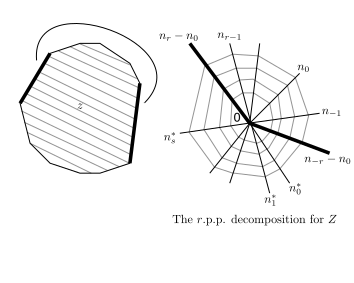
\includegraphics{vol58-fig/fig58-82.eps} 
\end{figure}
\end{prop}

\begin{remark*}
Unlike\pageoriginale Theorem \ref{chap2:thm14.3}, $Y$ and $Z$ may be
singular in 
general. They are non-singular if $r=1$. For each specific $N$, we can
certainly replace $Y$ by a blow up to obtained non-singular $Y$ and
$\pi^{-1}(0)$ consisting of non-singular components crossing
normally. As is obvious from the construction of $Y$ below, there,
many other choices for $Y$.     
\end{remark*}

\begin{proof}
As before, let $\tilde{N}=N \oplus \mathbb{Z}\ell$. Left the action of
$U^*_N$ on $N$ to $\tilde{N}$ by letting it act as the identity for
$\ell$. By Proposition \ref{chap2:prop15.2}, we have 
$$
n_0=1, \quad n_{-1}=\omega, \quad n^*_{-1}=\omega -1.
$$
This fact guarantees that $(\tilde{N}, \tilde{\Delta})$ is a
$U^*_N$-invariant r.p.p.decomposition, where $\tilde{\Delta}$
consists of the faces of 
\begin{align*}
\mathbb{R}_o(n_{ir}+\ell) &+ \mathbb{R}_on_{ir+v-1}+\mathbb{R}_on_{ir+v}  &i
\in \mathbb{Z} , \quad  0 \le v < r\\ 
\mathbb{R}_o(n_{ir}+\ell) &+ \mathbb{R}_o n^*_{is+v}+\mathbb{R}_o
n^*_{is+v+1}  &i \in \mathbb{Z} , \quad 0 \le v < s\\ 
\mathbb{R}_o(n_{ir}+\ell) &+  \mathbb{R}_o(n_{(i+1)r}+\ell)+
\mathbb{R}_on_{(i+1)r-1}  &i \in  \mathbb{Z}\\ 
\mathbb{R}_o(n_{ir}+\ell) &+ \mathbb{R}_o(n_{(i+1)r}+\ell)+
\mathbb{R}_o n^*_{(i+1)s} & i\in  \mathbb{Z}. 
\end{align*}

Seen from above the north pole, the decomposition induced by
$\tilde{\Delta}$ on a sphere in $\tilde{N}_\mathbb{R}$ centered at 0
looks like the picture below. 

Let $B$ be $\ord^{-1}$ of the union in $Mc(\tilde{N}, \tilde{\Delta})$
of $(\mathbb{R}_{>0} \times \mathbb{R}) \times \mathbb{R} \ell$ and
the boundary at infinity. Then $B$ is $U^+_N$-invariant and the action
is properly discontinuous without fixed point. By Theorem
\ref{chap1:thm4.2} (iii), we are done.  
\begin{figure}[H]
\centering 
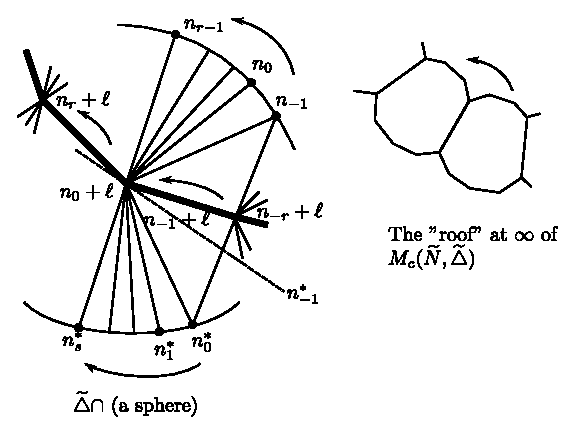
\includegraphics{vol58-fig/fig58-83.eps} 
\end{figure}
\end{proof}\pageoriginale

\begin{examples*}
\begin{enumerate}[(1)]
\item If $\omega =2 + \sqrt{3}=[[\bar{4}]]$, then $\omega^*=1+
  \sqrt{3}/3=[[\overline{2,3}]]$. Hence $X_N$ is as in the picture. We
  have 
\begin{align*}
n_1 & = -\omega +4, n_0=1,n_{-1}=\omega, n_{-2}=4 \omega -1\\
n^*_2 & = 2 \omega-7, n^*_1=\omega-3, n^*_0=\omega-2, n^*_{-1}=\omega-1,
n^*_{-2}=2 \omega -1. 
\end{align*}
Since $r=1$, $Y$ and $Z$ of Prop. \ref{chap2:prop15.7} are
non-singular. Taking the 
$U^+_N$-translates of $\mathbb{R}_o(n_0+
\ell)+\mathbb{R}_on_o+\mathbb{R}_on_1$ and $\mathbb{R}_o(n_0+
\ell)+\mathbb{R}_o(n_1+\ell)+\mathbb{R}_on_1$ instead of
$\mathbb{R}_o(n_0+ \ell)+\mathbb{R}_o(n_1+ \ell)+\mathbb{R}_on_0$ and
$\mathbb{R}_o(n_0+\ell)+\mathbb{R}_on_{-1}+\mathbb{R}_on_0$, we get a
different degeneration $Z'$  
\begin{figure}[H]
\centering 
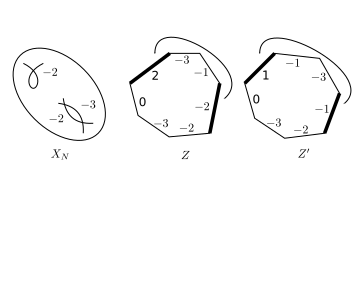
\includegraphics{vol58-fig/fig58-84.eps} 
\end{figure}

\item Let\pageoriginale $\omega = (3 + \sqrt{5}) /2 = [[\bar{3}]] =
  \omega^*$. Then $U_N$ is generated by $(-1 +\sqrt{5})/2$. Kato
  showed that the only possible configurations of curves for a minimal
  surface with $b_2 = 1$ and with a global spherical shell are that of
  $\hat{X_N}$ here as well as those in Theorem \ref{chap2:thm14.2} (i) and (ii). 

In this case, we have 
\begin{align*}
n_1 & = 3 - \omega , n_0  = 1, n_{-1} = \omega \\ 
n^*_1 & =  2\omega -5, n^*_0 = \omega -2, n^*_{-1} = \omega -1. 
\end{align*}

Again $Y$ and $Z$ of Prop. \ref{chap2:prop15.7} are non-singular in
this case. By a modification as in (1) above, we get a different
$Z'$. 
\begin{figure}[H]
\centering 
\includegraphics{vol58-fig/fig58-85.eps} 
\end{figure}

\item If $\omega = (3 + \sqrt{7} ) /2 = [[\bar{3,6}]] $, then $\omega^* =
  (5 + \sqrt{7}) / 3 = [ [\bar{3, 3, 2, 2, 2}] ]$. 
\end{enumerate}
\begin{figure}[H]
\centering 
\includegraphics{vol58-fig/fig58-86.eps} 
\end{figure}
\end{examples*}


\begin{thebibliography}{99}
\bibitem{keyA1} {K. Akao}\pageoriginale On prehomogeneous compact
  Kahler manifolds, in   \textit {Manifolds-Tokyo 1973} (Hattori,
  ed.), Univ.of Tokyo   Press, 1975, 365-371  

\bibitem{keyA2} {K.Akao}, Complex structure on $S^{2p+1} \times S^{2q+1}$
  with algebraic codimension 1, in \textit{Complex Analysis and
    Algebraic Geometry} (Baily and Shioda, eds.), Iwanami Shoten and
  Cambridge Univ.Press, 1977, 205-225 

\bibitem{keyB1} {A. Borel}, Linear algebraic groups, Benjamin, New York,
  1969 

\bibitem{keyBS} {A.Borel and J.-P.Serre}, Corners and arithmetic
  groups, Comm.Math.Helv. 48 (1973), 436-491 

\bibitem{keyC1} {P.Cartier}, Questions de ratinalit\'e des diviseurs en
  g\'eom\'etrie alg\'ebrique, Bull.Soc.Math.France, 86 (1958), 177-251
  \textit{Appendice}
 
\bibitem{keyC2}{H.Cohn}, Support polygon and the resolution of modular
  functional singularities, Acta Arithmetica, 24 (1973), 261-278 

\bibitem{keyD1} {C.Delorme}, Sous-mono\"ides d'intersection compl\'ete
  de $N$, Ann.Sci.Ecole Norm.Sup., 9 (1976), 145-154 

\bibitem{keyD2} {M. Demazure}, Sous-groupes alg\'ebriques de rang
  maximum du groupe de Cremona, Ann.Sci.Ecole Norm.Sup. 3 (1970),
  507-588 

\bibitem{keyDM} {P.Deligne and D.Mumford}, The irreduciblility of the
  space of curves\pageoriginale of given genus, Publ.Math.IHES, 36
  (1969), 75-110   

\bibitem{keyEGA} {A. Grothendieck and J.Dieudonn\'e}, \'El\'ement de
  g\'eom\'etrie  algebrique, Publ.Math.IHES,
  4, 8, 11, 17, 20, 24, 28, 32 (1960-1967)  

\bibitem{keyG1} {L.Gerritzen}, On non-archimedean representations of
  abelian varieties, Math.Ann. 196 (1972), 323-346 

\bibitem{keyG2} {G.Gonzalez-Sprinberg}, Eventails en dimension 2 et
  transforme de Nash, Centre de Math. Ecole Norm.Sup. Equipe de
  Rech.Assoc. au CNRS  No.589, Fev.1977. 

\bibitem{keyG3}{B.Gr\"unbaum}, \textit{Convex polytopes}, Interscience,
  New York, 1967 

\bibitem{keyG4}{B.Gr\"unbaum}, Polytopes, graphs, and complexes, Bull.
  Amer. Math. Soc., 76 (1970),  1131-1201 

\bibitem{keyGG} {L.Gerritzen and H.Grauert}, Die Azyklizit\"at der
  affinoiden Uberdeckung, in \textit{Global Analysis} (Iyanaga and
  Spencer, eds.), Univ.of Tokyo Press and Princeton Univ.Press,
1969,  159-184 

\bibitem{keyH1} {R.Hartshorne}, \textit{Ample subvarieties of algebraic
  varieties}, Lecture Notes in Math. 156, Springer-Verlag, 1970
 
\bibitem{keyH2} {J.Herzog}, Generators and relations of abelian semigroups
  and semigroup rings, Manuscripta Math. 3 (1970), 175-193
 
\bibitem{keyH3} {H.Hironaka}, Resolution of singularities of an algebraic
  variety\pageoriginale over a field of characteristic zero, I-II,
  Ann.of Math. 79 (1964), 109-326  

\bibitem{keyH4} {F.Hirzebruch}, Hilbert modular surface, L'enseignement
  Math. 21 (1973), 183-282 

\bibitem{keyH5} {M.Hochster}, Rings of invariants of tori, Cohen-Macaulay
  rings generated by monomials, and polytopes, Ann.of  Math. 96 
  (1972), 318-337
 
\bibitem{keyHK} {J.Herzog and E.Kunz}, Die Wertehalbgruppe eines lokalen
  Rings der Dimension 1, Sitzungsberichte der Heidelberger Akad.der
  Wiss., 2.Abh., Springer-Verlag, 1971 

\bibitem{keyI1} {M.Inoue}, On surface of class $VII_0$, Inventiones math.
  24 (1974), 269-310
 
\bibitem{keyI2} {M.Inoue}, New surfaces with no meromorphic functions, in
  \textit{Proceedings of the  Intern. Congress of Math}., Vancouver
 1974,  vol.1, 423-426 

\bibitem{keyI3} {M.Inoue}, New surfaces with no meromorhic functions,
  II, in \textit{Complex Analysis and Algebraic Geometry} (Baily
  and Shioda, eds.), Iwanami Shoten and Cambridge Univ.Press, 1977,
  91-106 

\bibitem{keyI4} {M.Ishida}, Graded factorial rings of diemension 3 of a
  mesticted bype, to appear in J.Math.Kyoto Univ.
 
\bibitem{keyI5} {M.Ishida}, Compactifications of a family of generalized
  Jacobian varieties, to appear in the \textit{Proceedings of  the
    Intern.Symp.on Alg.Geom., Kyoto 1977}
 
\bibitem{keyI6} {B.Iversen,}\pageoriginale $A$ fixed point formula for
  action of tori on algebraic varieties, Inventiones math. 16
  (1972), 229-236  
 
\bibitem{keyK1} {T.Kaneyama,} On equivariant vector bundles on an almost
  homogeneous variety, Nogoya Math.J. 57 (1975), 65-86 
 
\bibitem{keyK2} {Ma.Kato,} Complex manifolds containing ``global''
  spherical shell, $I$, to appear in the \textit{Proceedings of the
    Intern.Symp.on  Alg.Geom., Kyoto 1977}
 
\bibitem{keyK3} {K.Kodaira,} On the structure of compact complex analytic
  surfaces  

\begin{tabular}{rlll}
 I &  Amer. J. Math. & 86 (1964), &751-798\\
 II & ibid. & 88 (1966), & 682-721\\
 III & ibid. & 90 (1968), & 55-83\\
 IV & ibid. &&  1048-1066
\end{tabular}

See also \text{Kunihiko Kodaira Collected Works,} Vol.III Iwanami
Shoten and Princeton Univ. Press, 1975 

\bibitem{keyK4} {K.Kodaira,} Holomorphic mappings of polydiscs into
  compact complex manifolds, J.Diff. Geom. 6 (1971), 33-46  

\bibitem{keyM1} {T.Mabuchi,} Almost homogeneous torus actions on varieties
  with ample tangent bundle, to appear in Tohoku Math. J. 

\bibitem{keyM2} {J.McCabe,} p-adic theta functions, thesis Harvard
  Univ.1968   

\bibitem{keyM3} {S.Mori}, On a generalization of complete
  intersections, J. Math. Kyoto Univ. 15 (1975), 619-646 

\bibitem{keyM4} {S.Mori,} Graded factorial domains, to appear in
  J.Math. Kyoto Univ.
 
\bibitem{keyM5} {H.Morikawa,}\pageoriginale Theta functions and
  abelian varieties over valuation fields of rank one, I-II,
  Nagoya Math.J. 20(1962), 1-27 and 21(1962), 231-250
 
\bibitem{keyM6} {J.Morrow,} Minimal normal compactifications of
  $\mathbb{C}^2$, Rice Univ.Studies 59 (1973), 97-112 

\bibitem{keyM7} {D.Mumford,} An analytic construction of degenerating
  abelian varieties over complete rings, Compositio
  Math. 24 (1972), 239-272
 
\bibitem{keyM8} {D.Mumford,} Introduction to algebraic geometry,
  mimeographed notes, Harvard Univ.
 
\bibitem{keyMO} {K.Miyake and T.Oda,} Almost homogeneous algebraic
  varieties under algebraic torus action, in \textit{Manifolds-Tokyo
    1973} (Hattori,ed.), Univ.of Tokyo Press, 1975, 373-381
 
\bibitem{keyMS} {S.Mori and H.Sumihiro,} On Hartshorne's conjecture, to
  appear in J.Math.Kyoto Univ. 

\bibitem{keyN1} {M.Nagata,} On rational surfaces, I-II, Memoirs
  Coll.Sci. Univ.Kyoto, 32 (1960), 351-370 and 33 (1960), 271-293 

\bibitem{keyN2} {O.Nagaya,} Classification of 3-dimensional complete
  non-singular torus embeddings, Master's thesis, Nagoya Univ. 1976
 
\bibitem{keyN3} {I.Nakamura,} On moduli of stable quasi-abelian varieties,
  Nagoya Math.J. 58(1975), 149-214

\bibitem{keyN4} {I.Nakamura,} Relative compactification of the Neron model
  and its applications, in \textit{Complex Analysis and Algebraic
    Geometry}\pageoriginale (Baily and Shioda,eds.),Iwanami Shoten and
  Cambridge   Univ.Press, 1977,205-225 

\bibitem{keyN5} {Y.Namikawa,} A new compactification of the Siegel space
  and the degeneration of abelian varieties, I-II,
  Math.Ann. 221 (1976), 97-141 and 201-241

\bibitem{keyN6} {Y.Namikawa,} Toroidal degeneration of abelian varieties,
  in  \textit{Complex Analysis and Algebraic Geometry} (Baily and
  Shioda, eds.), Iwanami Shoten and Cambridge
  Univ.Press, 1977, 227-237

\bibitem{keyO1} {P.Olum,} Non-abelian cohomology and van Kampen's theorem,
  Ann.of Math.  68 (1958), 658-668

\bibitem{keyOS} {T.Oda and C.S.Seshadri,} Compactifications of the
  generalized Jacobian variety, to appear in Transactions
  Amer.Math.Soc.

\bibitem{keyOW} {P.Orlik and P.Wagreich,} Algebraic surfaces with
  $k^*$-action, to appear

\bibitem{keyP1} {O.Perron,} \textit{Die Lehre von Kettenbr\"unchen, }
  B.G.Teubner, Leipzig und Berlin, 1913

\bibitem{keyP2} {V.L.Popov,} Quasi-homogeneous affine algebraic
  varieties of the group SL(2), Izv.Akad.Nauk SSSR
  37 (1973), 792-832 = Math.USSR Izv. 7 (1973), 793-831

\bibitem{keyP3} {V.L.Popov,} Classification of 3-dimensional affine
  algebraic varieties that are quasi-homogeneous with respect to an
  algebraic group, Izv.Akad.Nauk.SSSR 39 (1975), 566-609 = Math.USSR
  Izv. 9 (1975), 535-576

\bibitem{keyR1} {M.Rapoport,}\pageoriginale Compactifications de $1'$
  espace de modules de Hilbert-Blumenthal,thesis Universite de
  Paris-Sud, 1976. 

\bibitem{keyR2} {M.Raynaud,} \textit{Faiscaux amples sur les schemas en
  groupes et les espaces homogenes}, Lecture Notes in Math. 119,
  Springer-Verlag, 1970

\bibitem{keyR3} {R.T.Rockafellar,} \textit{Convex analysis,} Princeton
  Univ.Press 1970

\bibitem{keyS1} {I.Satake,} On the arithmetic of tube domains,
  Bull.Amer.Math. Soc. 79 (1973), 1076-1094

\bibitem{keyS2} {R.R.Simha,} Algebraic varieties biholomorphic to
  $\mathbb{C}^* \times \mathbb{C}^*$, to appear in Tohoku Math.J.

\bibitem{keyS3} {H.Sumihiro,} Equivariant completion, I-II, J.Math.Kyoto
  Univ.14 (1974), 1-28 and 15 (1975), 573-605

\bibitem{keyS4} {T.Suma,} On hyperelliptic surfaces, J.Fac.Sci.Univ.Tokyo,
  16 (1970), 469-476

\bibitem{keySC} {A.Ash,} D.Mumford, M.Rapoport and Y.Tai,\textit{Smooth
  compcatification of locally symmetric varieties}, Lie Groups: History
  Frontiers and Applications IV, Math.Sci.Press, Brookline, Mass. 1975  

\bibitem{keyT1} {H.Tsuchihashi,} Degenerations of hyperelliptic surfacces,
  Master's thesis, Tohoku Univ., 1978

\bibitem{keyTE} {G.Kempf,} F.Knudsen, D.Mumford and B.Saint-Donat,
  \textit{Toroidal embeddings I}, Lecture Notes in Math. 339,
  Springer 1973 

\bibitem{keyU1} {T.Ueda,} to appear
\end{thebibliography}

